\documentclass[preprint,12pt,authoryear]{elsarticle}

\usepackage{amsmath,amssymb,amsfonts}
\usepackage{algorithm}
\usepackage{algpseudocode}
\usepackage{graphicx}
\usepackage{textcomp}
\usepackage{booktabs}
\usepackage{multirow}
\usepackage{hyperref}
\usepackage{pgfplots}
\pgfplotsset{compat=1.17}
\usepackage{tikz}
\usetikzlibrary{shapes.geometric,arrows.meta,positioning,fit}

\journal{Engineering Applications of Artificial Intelligence}

\begin{document}

\begin{frontmatter}

\title{Retrieval-augmented large language models for training-free trajectory reconstruction under satellite navigation spoofing in aviation and maritime surveillance}

\author[bgu]{Yuval Felendler\corref{cor1}}
\ead{yuvalfel@post.bgu.ac.il}
\author[bgu]{Ruben Sasson}
\ead{rubenyaa@post.bgu.ac.il}
\author[bgu]{Yuval Elovici}
\ead{elovici@bgu.ac.il}
\author[bgu]{Asaf Shabtai}
\ead{shabtaia@bgu.ac.il}

\cortext[cor1]{Corresponding author.}
\address[bgu]{Faculty of Computer and Information Science, Ben-Gurion University of the Negev, Beer-Sheva, Israel}

\begin{abstract}
When an aircraft or a vessel is suspected of receiving spoofed satellite-navigation
signals, surveillance operators must discard its broadcast positions yet keep
tracking it. Existing trajectory predictors are trained for a single transport
domain and must be rebuilt for each new one. This paper extends TrajRAG
(Trajectory Retrieval-Augmented Generation) from aviation to a domain-agnostic
framework. \emph{Contribution in artificial intelligence:} we formulate
post-detection trajectory reconstruction as retrieval-conditioned sequential
inference by a large language model whose parameters are never updated, and we
isolate a domain adapter -- a textual-state prompt template, a phase-indexed
vector memory, a trusted non-satellite signal and a data-calibrated kinematic
feasibility bound -- as the only component that changes between domains.
\emph{Application in engineering:} one reconstruction engine maintains track
continuity for air-traffic surveillance based on Automatic Dependent
Surveillance--Broadcast messages and for vessel traffic services based on
Automatic Identification System messages. Transferred to shipping without any
model training, the framework is evaluated on commercial vessels in two
United States port corridors, against a retrieval memory that structurally
excludes both the test set and any chronologically later voyage, and against
fourteen maritime baselines. It reduces mean reconstruction error by a factor
of 1.3--1.5 relative to the best classical baseline in every voyage phase,
significantly so (paired Wilcoxon test, $p<10^{-3}$ in every case). Against a
trained, ship-specific convolutional network, it is statistically
indistinguishable in every phase (Houston, $n=50$), matching -- without any
maritime training data -- a model purpose-trained on this corridor's own
traffic. A complete blackout reconstruction finishes in under 35\,s, well
within the 5-minute vessel reporting interval. These results show that prompt
and memory design, rather than retraining, can carry trajectory reconstruction
across transport domains.
\end{abstract}

\begin{highlights}
\item Training-free trajectory reconstruction after satellite-navigation spoofing
\item One engine serves aircraft and ships; only prompt, index and trusted signal change
\item Ship trajectories reconstructed with a frozen language model and no ship training
\item Statistically indistinguishable from a trained, ship-specific network in every phase tested
\item Significantly beats every classical, recurrent and retrieval-only baseline; validated on 1,544 flights and 60 vessels against fourteen maritime baselines
\end{highlights}

\begin{keyword}
Satellite navigation spoofing \sep Trajectory reconstruction \sep Retrieval-augmented generation \sep Large language models \sep Automatic Identification System \sep Air traffic surveillance \sep Cross-domain transfer
\end{keyword}

\end{frontmatter}

\section{Introduction}
\label{sec:intro}

Aircraft and ships are tracked by cooperative surveillance systems that
rebroadcast positions computed by an on-board Global Navigation Satellite
System (GNSS) receiver. In aviation the carrier is Automatic Dependent
Surveillance--Broadcast (ADS-B) \citep{faa2007adsb,khan2025adsbsurvey}; at sea
it is the Automatic Identification System (AIS) \citep{itu2014ais}. Neither
channel authenticates the position it carries, so a receiver that is jammed
or spoofed passes the corrupted position directly to air traffic control
(ATC) and vessel traffic services (VTS). Interference has become a routine
operational condition rather than a rare event. Aviation monitoring reports a
sustained rise in GNSS anomalies in and around conflict zones
\citep{aireon2025,felux2025navigating,ieropoulos2024impact,lo2025observations}.
Maritime trackers reported roughly 700 jamming and spoofing events per day
across the global fleet in 2024 \citep{windward2025}. In the Baltic Sea, the
number of affected vessels grew from about 1,225 in the first quarter of 2025
to more than 5,800 in the second \citep{gpspatron2025}. A single two-week
window in mid-2025 recorded more than 12,000 spoofing incidents involving
over 3,000 vessels \citep{kpler2025}, and sustained spoofing has been
documented in the Persian Gulf \citep{skuld2025,maritimeexec2025}.

Detecting interference is necessary but not sufficient. Once a detector
flags an aircraft or a vessel, its satellite-derived positions must be
discarded, yet the operator still has to deconflict traffic, enforce
separation and verify that the asset stays clear of restricted areas. In a
narrow ship channel or a busy terminal area, losing a reliable track for
even half an hour is operationally significant. The engineering problem is
therefore \emph{post-detection reconstruction}: estimating where the asset is
from its last trusted state, from signals that do not depend on satellites,
and from what similar assets have done before.

Today this gap is usually filled by trajectory predictors used as
extrapolators. These predictors are almost always domain-specific. Aircraft
predictors are trained on flights \citep{pang2019lstm,kwak2025evolution}, and
vessel predictors are trained on AIS voyages
\citep{li2023ship,shin2024aisacnet,nguyen2024transformer}. Each must be
rebuilt, retuned and revalidated when it is moved to a new region, a new
traffic mix or a new transport mode. For an organisation that operates both
airspace and coastal surveillance, or for a vendor that supplies both, this
means maintaining two unrelated model families for what is essentially the
same task.

In the conference version of this work \citep{felendler2026trajrag} we
introduced TrajRAG for aircraft. TrajRAG converts trajectory segments into
textual state descriptions and stores them in phase-specific vector indices.
During a blackout it retrieves phase-consistent historical segments and lets
a large language model (LLM) propose the next position, which is accepted
only inside a kinematic feasibility envelope. That study was limited to
aviation: it did not establish whether the design is specific to aircraft
dynamics and ADS-B, or whether it is a reusable reconstruction method. This
paper answers that question. Our thesis is that \emph{nothing in the
reconstruction engine needs to be learned per domain}: moving to a new
transport mode should require only a new prompt template, a new retrieval
index and a small set of physically motivated constants, all derived from
domain data by fixed procedures.

We test this thesis on shipping, which differs from aviation in almost
every respect that matters to a predictor. Vessels are an order of
magnitude slower. AIS is sampled irregularly. Phase dynamics are dominated
by berthing manoeuvres rather than altitude changes, the environmental
drivers are currents and waves rather than winds aloft, and the
GNSS-independent signal available on board is different. If the same
engine, with its LLM frozen and no maritime gradient update, competes with
dedicated maritime models, the result is evidence that retrieval and
prompting can replace retraining in this class of engineering problem.

\paragraph{Contributions} The contributions of this paper are:
\begin{enumerate}
\item \textbf{A domain-agnostic formulation (AI contribution).} We separate
post-detection reconstruction into a shared engine (retrieval, frozen-LLM
proposal, feasibility guard and feedback loop) and a domain adapter of eight
elements. We specify the adapter formally and show that it is the only part
that changes between aviation and shipping (Section~\ref{sec:framework}).
\item \textbf{A maritime instantiation built without training.} We
construct the maritime adapter (AIS state schema, gyrocompass heading as the
trusted signal, departure/transit/arrival phases, marine environmental
context and a voyage prompt template), together with a new public-data
corpus of 3,506 voyages from 26.2 million AIS reports in two United States
port corridors (Sections~\ref{sec:instantiation} and
\ref{sec:data}).
\item \textbf{A rigorous maritime benchmark.} We compare against fourteen
baselines: classical, recurrent, retrieval-only, seven modern forecasters and
AIS-ACNet, a trained ship-specific network published in this journal
\citep{shin2024aisacnet}. All are run on a common held-out test set with
paired significance tests and distance- and time-normalised errors
(Section~\ref{sec:results}).
\item \textbf{A transferable calibration procedure for the feasibility
guard.} We show that the procedure used to calibrate the guard transfers
across domains, while the constant it produces does not. Vessel dynamics
give a phase-dependent displacement-ratio distribution with no counterpart
in aviation (Section~\ref{sec:calibration}).
\item \textbf{A real-time dual-domain system design.} We describe how one
deployment serves ATC and VTS, and we show that the reconstruction latency
fits inside the reporting interval of both surveillance channels
(Sections~\ref{sec:architecture} and \ref{sec:latency}).
\end{enumerate}

\paragraph{Relation to the conference version} The conference paper
\citep{felendler2026trajrag} covers aviation only. The domain-adapter
formulation, the maritime instantiation and corpus, the full maritime
evaluation (fourteen baselines, normalised errors, significance tests and
corridor analysis), the cross-domain calibration analysis and the
dual-domain system architecture are new. Aviation results are summarised in
Section~\ref{sec:aviation-reference} only as the reference point for the
cross-domain comparison; we do not repeat the aviation ablations, backbone
study or real-world case studies, and refer the reader to the conference
paper for them.

The rest of the paper is organised as follows. Section~\ref{sec:related}
reviews related work. Section~\ref{sec:framework} presents the
domain-agnostic framework and the system architecture. Section~\ref{sec:instantiation}
describes the two instantiations. Section~\ref{sec:design} details the
experimental design, and Section~\ref{sec:results} reports the results.
Section~\ref{sec:discussion} discusses implications and threats to validity,
and Section~\ref{sec:conclusion} concludes.

\section{Related work}
\label{sec:related}

\subsection{Satellite-navigation interference in transport surveillance}

ADS-B horizontal position and velocity are derived from the aircraft's GNSS
receiver, so interference propagates directly into the surveillance picture
\citep{khan2025adsbsurvey,pik2024detecting,pik2025gps}. AIS has the same
weakness: position, SOG and COG are GNSS-derived and broadcast over an
unauthenticated VHF link \citep{itu2014ais}. Most research addresses
\emph{detection}. In aviation, studies correlate ADS-B position gaps and
integrity indicators with notices to airmen \citep{pik2024detecting}. At
sea, recent work uses AIS as a sensor of opportunity to detect and localise
interference over wide areas \citep{park2026aisbased,winkel2026seaspoof},
and recurrent classifiers flag spoofed AIS points \citep{raj2025vessel}.
These detectors decide \emph{when} a track can no longer be trusted. Our
work starts at that point and addresses what the operator sees
\emph{after} the decision.

\subsection{Trajectory prediction and reconstruction}

Classical trackers such as Kalman and interacting-multiple-model filters
\citep{kalman1960new,ren2024improved} work well over short horizons. Under
interference, however, corrupted measurements are discarded rather than
smoothed, so the filter runs open loop and its error grows with the gap.
Autoregressive models behave similarly. Recurrent networks
\citep{pang2019lstm,hashemi2024bidirectional} capture non-linear motion but
depend on training coverage and drift without feedback. Recent reviews of
aircraft \citep{kwak2025evolution} and ship trajectory prediction
\citep{li2023ship,guo2026systematic} describe a mature but domain-siloed
literature dominated by recurrent, convolutional, attention-based and hybrid
networks. Among maritime models, AIS-ACNet \citep{shin2024aisacnet} couples
parallel dilated-convolution encoders for position and for auxiliary SOG/COG
targets and was evaluated on Port of Houston AIS. Because it predicts
forward only and has public code, it is the most suitable literature
baseline for our protocol. TrAISformer \citep{nguyen2024transformer}
discretises AIS states and predicts them with a transformer. Generic
forecasters such as DLinear \citep{zeng2023transformers}, PatchTST
\citep{nie2023timeseries}, iTransformer \citep{liu2024itransformer}, Informer
\citep{zhou2021informer}, Autoformer \citep{wu2021autoformer}, FEDformer
\citep{zhou2022fedformer} and TimesNet \citep{wu2023timesnet} provide strong
domain-independent baselines, but each must be trained on target data.

A separate line of work imputes ordinary AIS coverage gaps. MH-GIN
\citep{liu2026mhgin} uses multi-scale heterogeneous graphs. HABIT
\citep{spiliopoulos2026habit} uses historical hexagon transitions and path
search. VISTA \citep{liu2026vista} lets an LLM choose an imputation pattern
from a knowledge graph built from historical counts, which gives each repair
a readable provenance. These methods are the closest to ours in spirit, but
they interpolate between two known endpoints and address benign gaps. Our
setting is forward-only: the end of the blackout is unknown, and the
positions inside it are deliberately discarded.

\subsection{Large language models and retrieval for temporal data}

LLMs can forecast numeric series zero-shot when values are serialised as
text \citep{gruver2023large}, and they can be reprogrammed for forecasting
with a small trained adapter \citep{jin2024timellm}. Retrieval-augmented
generation grounds a parametric model in non-parametric memory
\citep{lewis2020retrieval}, and TS-RAG \citep{ning2025tsrag} shows that
retrieval improves zero-shot time-series foundation models. For flights,
LLMs have been fine-tuned on serialised ADS-B states \citep{luo2025large}
and assessed qualitatively for reconstruction \citep{zhang2024exploratory}.
None of these approaches encodes the constraints that make trajectory
reconstruction safe to deploy: operational phase, a trusted signal that is
physically independent of the corrupted one, and a hard bound on feasible
displacement. None of them has been shown to move between transport domains
without retraining.

\subsection{Positioning}

Table~\ref{tab:positioning} summarises where this work sits. Its
distinguishing combination is a post-detection, forward-only formulation, no
target-domain training, an explicit physical guard and a demonstrated
transfer across two physically distinct transport domains.

\begin{table}[t]
\centering
\caption{Positioning of this work relative to representative
trajectory-prediction and reconstruction approaches. ``Post-detection''
means that horizontal positions after the onset are withheld rather than
denoised. ``No training'' means that no model parameters are fitted on
target-domain trajectories.}
\label{tab:positioning}
\footnotesize
\begin{tabular}{p{3.0cm}ccccc}
\toprule
Approach & Post-det. & No training & Phys. guard & Multi-domain & Interpretable \\
\midrule
Kalman / IMM filters & \checkmark & \checkmark & -- & \checkmark & -- \\
Recurrent/conv. predictors & -- & -- & -- & -- & -- \\
Generic time-series forecasters & -- & -- & -- & -- & -- \\
AIS imputation (MH-GIN, VISTA, HABIT) & -- & partly & -- & -- & partly \\
Fine-tuned LLM flight prediction & -- & -- & -- & -- & \checkmark \\
Zero-shot/retrieval LLM forecasting & -- & \checkmark & -- & \checkmark & -- \\
TrajRAG, aviation only \citep{felendler2026trajrag} & \checkmark & \checkmark & \checkmark & -- & \checkmark \\
\textbf{This work} & \checkmark & \checkmark & \checkmark & \checkmark & \checkmark \\
\bottomrule
\end{tabular}
\end{table}

\section{Domain-agnostic reconstruction framework}
\label{sec:framework}

\subsection{Problem formulation}
\label{sec:problem}

Let $X = \{x_0, \ldots, x_n\}$ be a time-ordered trajectory of an aircraft or
a vessel. Each state $x_i = (y_i, k_i, a_i, \mathrm{time}_i)$ contains a
horizontal position $y_i = (\phi_i, \lambda_i)$, kinematic fields $k_i$ (for
example ground speed and track, or SOG and COG) and the reading $a_i$ of a
trusted auxiliary signal. The trusted signal must be \emph{physically}
independent of the satellite receiver, not merely reported in a separate
field. An external detector raises an alarm at index $t$. From then on,
every satellite-derived field ($y_i$ and the satellite-derived part of
$k_i$, for $i > t$) is withheld from the reconstruction, while $a_i$ remains
available. The task is to produce
\begin{equation}
\hat{Y}_{t+1:r} = \{\hat{y}_i\}_{i=t+1}^{r}
\label{eq:task}
\end{equation}
until trusted reporting resumes, or the trip ends, at index $r$. The
available information is the verified prefix $X_{0:t}$, the trusted signal
$a_{0:r}$, environmental context obtained independently of the asset, and
historical trajectories of the same domain. This is not denoising, because
corrupted observations are dropped rather than filtered. It is not
interpolation either, because the end state is unknown. We evaluate it as
forward-only reconstruction against the true, uncorrupted positions.

\subsection{Shared engine and domain adapter}

We factor the method into a shared engine and a domain adapter. The
\emph{engine} comprises a frozen text-embedding model $g$, a frozen LLM $f$,
an inner-product vector index, the iterative propose--validate--update loop
of Algorithm~\ref{alg:reconstruction}, the feasibility guard and a fixed
output schema (one latitude/longitude pair per step). No component of the
engine is trained, fine-tuned or adjusted for a domain. A domain adapter is
the tuple
\begin{equation}
\mathcal{D} = \langle \mathcal{S}, a, \mathcal{P}, \pi, \tau, \mathcal{E}, \mathcal{M}, \kappa \rangle,
\label{eq:adapter}
\end{equation}
whose elements are:
\begin{itemize}
\item $\mathcal{S}$, the \emph{state schema}, which lists the fields of a
surveillance report and marks each as satellite-derived (untrusted after
onset) or trusted;
\item $a$, the \emph{trusted auxiliary signal};
\item $\mathcal{P}$ and $\pi$, the \emph{phase taxonomy} and a
phase-assignment rule that uses only trusted information;
\item $\tau$, the \emph{verbaliser}, a prompt template that turns a
trajectory segment, the trusted signal and the environmental context into a
short textual state description;
\item $\mathcal{E}$, the \emph{environmental context provider}, queried at
the last accepted (trusted or reconstructed) position and time;
\item $\mathcal{M} = \{\mathcal{M}_p\}_{p \in \mathcal{P}}$, the
\emph{phase-indexed memory}, built by applying $\tau$ and $g$ to historical
trajectories of the domain;
\item $\kappa = (\Delta t, \{\alpha_p\}, \mathrm{SPEEDRULE})$, the
\emph{kinematic constants}: the sampling interval, per-phase tolerance
factors and the rule that updates the reference speed during a blackout.
\end{itemize}
Three of these elements are semantic choices that a domain expert makes
once: the trusted signal, the phase taxonomy and the vocabulary of the
verbaliser. The remaining elements are data artefacts produced from the
domain corpus by procedures that are identical in both domains
(Sections~\ref{sec:offline-memory} and \ref{sec:calibration}). Porting the
method to a new domain therefore requires a prompt template, an index and a
calibration run. It requires no training run.

\begin{algorithm}[t]
\caption{Online reconstruction with the shared engine and a domain adapter $\mathcal{D}$}
\label{alg:reconstruction}
\begin{algorithmic}[1]
\Require verified prefix $X_{0:t}$; trusted signal $a_{0:r}$; adapter
$\mathcal{D} = \langle \mathcal{S}, a, \mathcal{P}, \pi, \tau, \mathcal{E}, \mathcal{M}, \kappa \rangle$
with $\kappa = (\Delta t, \{\alpha_p\}, \mathrm{SPEEDRULE})$; frozen LLM $f$;
frozen encoder $g$; retrieval size $K$
\Ensure reconstructed positions $\hat{Y}_{t+1:r}$
\State $p \gets \pi(X_{0:t}, a_{0:t})$ \Comment{phase from trusted information only}
\State $(\hat{y}_t, v) \gets (y_t, v_t)$ \Comment{last verified position and speed}
\State $q \gets \tau(X_{0:t}, a_{0:t}, (\hat{y}_t, t))$ \Comment{textual state of the prefix}
\For{$i = t+1, \ldots, r$}
  \State $C \gets \mathrm{TopK}(g(q), \mathcal{M}_p, K)$ \Comment{cosine similarity}
  \State $\tilde{y}_i \gets f(q, C, a_i, (\hat{y}_{i-1}, i))$ \Comment{fixed schema: latitude, longitude}
  \State $d_{\max} \gets \alpha_p \, v \, \Delta t$
  \If{$d_{\mathrm{hav}}(\tilde{y}_i, \hat{y}_{i-1}) > d_{\max}$}
    \State $\tilde{y}_i \gets \mathrm{Project}(\tilde{y}_i, \hat{y}_{i-1}, d_{\max})$; raise low-confidence flag
  \EndIf
  \State $\hat{y}_i \gets \tilde{y}_i$
  \State $v \gets \mathrm{SPEEDRULE}(v, \hat{y}_{i-1}, \hat{y}_i, i)$ \Comment{domain-specific (Section~\ref{sec:instantiation})}
  \State $q \gets \tau(X_{0:t} \cup \hat{Y}_{t+1:i}, a_{0:i}, (\hat{y}_i, i))$ \Comment{feedback: re-query from reconstructed prefix}
\EndFor
\State \Return $\hat{Y}_{t+1:r} = \{\hat{y}_i\}_{i=t+1}^{r}$
\end{algorithmic}
\end{algorithm}

\subsection{Offline memory construction}
\label{sec:offline-memory}

Historical trajectories are cleaned (duplicates removed, timestamps made
monotonic), resampled to the adapter's $\Delta t$ when the native sampling
is irregular, and segmented into phases. Each segment is verbalised by
$\tau$ into a description of its spatial evolution, kinematic trend, phase,
elapsed time in phase and aligned environmental context. Timestamps are
expressed as time from the start of the phase so that segments recorded on
different days are comparable. Descriptions are embedded by $g$,
L2-normalised and stored in a separate inner-product index per phase (and,
in the maritime adapter, per corridor). Each index entry keeps a pointer to
the numeric continuation of its segment, which is shown to the LLM at
inference time. Separating indices by phase prevents incompatible motion
regimes, such as berthing and open-channel transit, from being retrieved
together. New data are added by appending entries, without re-fitting any
model.

\subsection{Online retrieval-conditioned reconstruction}

At onset, the phase is determined by $\pi$ from trusted information, and the
verified prefix is verbalised into a query. At each step the engine
retrieves the $K$ most similar segments from $\mathcal{M}_p$ by cosine
similarity. The LLM then receives the query, the retrieved segments with
their continuations, the trusted reading $a_i$ and the environmental
context, and returns the next position in the fixed schema. After the
position passes the guard, the query is rebuilt from the extended (verified
+ reconstructed) prefix, so the retrieved neighbours evolve as the
reconstruction progresses (Algorithm~\ref{alg:reconstruction}). The LLM thus
acts as a retrieval-conditioned \emph{proposal generator}: it adapts and
blends the retrieved precedents to the current context, but it never has the
final word on feasibility.

\subsection{Kinematic feasibility guard and its calibration procedure}
\label{sec:calibration}

Each proposal $\tilde{y}_i$ must lie within a disc centred at the last
accepted position, with radius
\begin{equation}
d_{\max} = \alpha_p \, v \, \Delta t,
\label{eq:guard}
\end{equation}
where $v$ is the current reference speed and $\alpha_p$ is a phase
tolerance. Proposals outside the disc are projected onto its boundary along
the bearing from the previous position, and the step is flagged as low
confidence. The guard therefore turns any LLM error, including a
hallucinated position, into a bounded displacement.

The tolerance is not tuned on reconstruction accuracy. It is set by a fixed,
accuracy-independent \emph{calibration procedure}. On the domain's training
trajectories we compute the step displacement ratio
\begin{equation}
\rho_i = \frac{d_{\mathrm{hav}}(y_{i-1}, y_i)}{v_{i-1} \, \Delta t},
\label{eq:rho}
\end{equation}
excluding steps with near-zero reference speed, and we set $\alpha$ to a
high quantile of $\rho$ (the 99th percentile in this study). For aircraft
this procedure gives $Q_{0.99}(\rho) = 1.18$ and hence $\alpha = 1.2$
\citep{felendler2026trajrag}. Section~\ref{sec:maritime-calibration} applies
the same procedure to vessels and shows why the procedure, rather than the
constant, is what transfers between domains.

\subsection{Real-time dual-domain system architecture}
\label{sec:architecture}

Fig.~\ref{fig:architecture} shows how the framework is deployed as one
service for both surveillance domains. ADS-B and AIS streams feed an
external spoofing detector, which this paper treats as a given interface.
When an alarm is raised for an asset, a trust gate stops forwarding that
asset's satellite-derived fields. The message type selects the domain
adapter. The shared engine then produces one reconstructed position per
reporting interval until the detector clears the alarm or the trip ends.
Each reconstructed position carries a confidence flag that records whether
the guard had to clamp the proposal, so a controller or VTS operator sees
the reconstruction together with an explicit indication of how far it
relies on the physical bound rather than on precedent. Because adapters
contain only prompts, indices and constants, a new domain or corridor is
added by deploying a new adapter. The engine, and any accreditation
evidence gathered for it, stays unchanged. Memories are refreshed by
appending completed trips, for example once a day.
Section~\ref{sec:latency} checks the latency of this loop against the
reporting interval of each channel.

\begin{figure}[t]
\centering
\resizebox{\linewidth}{!}{%
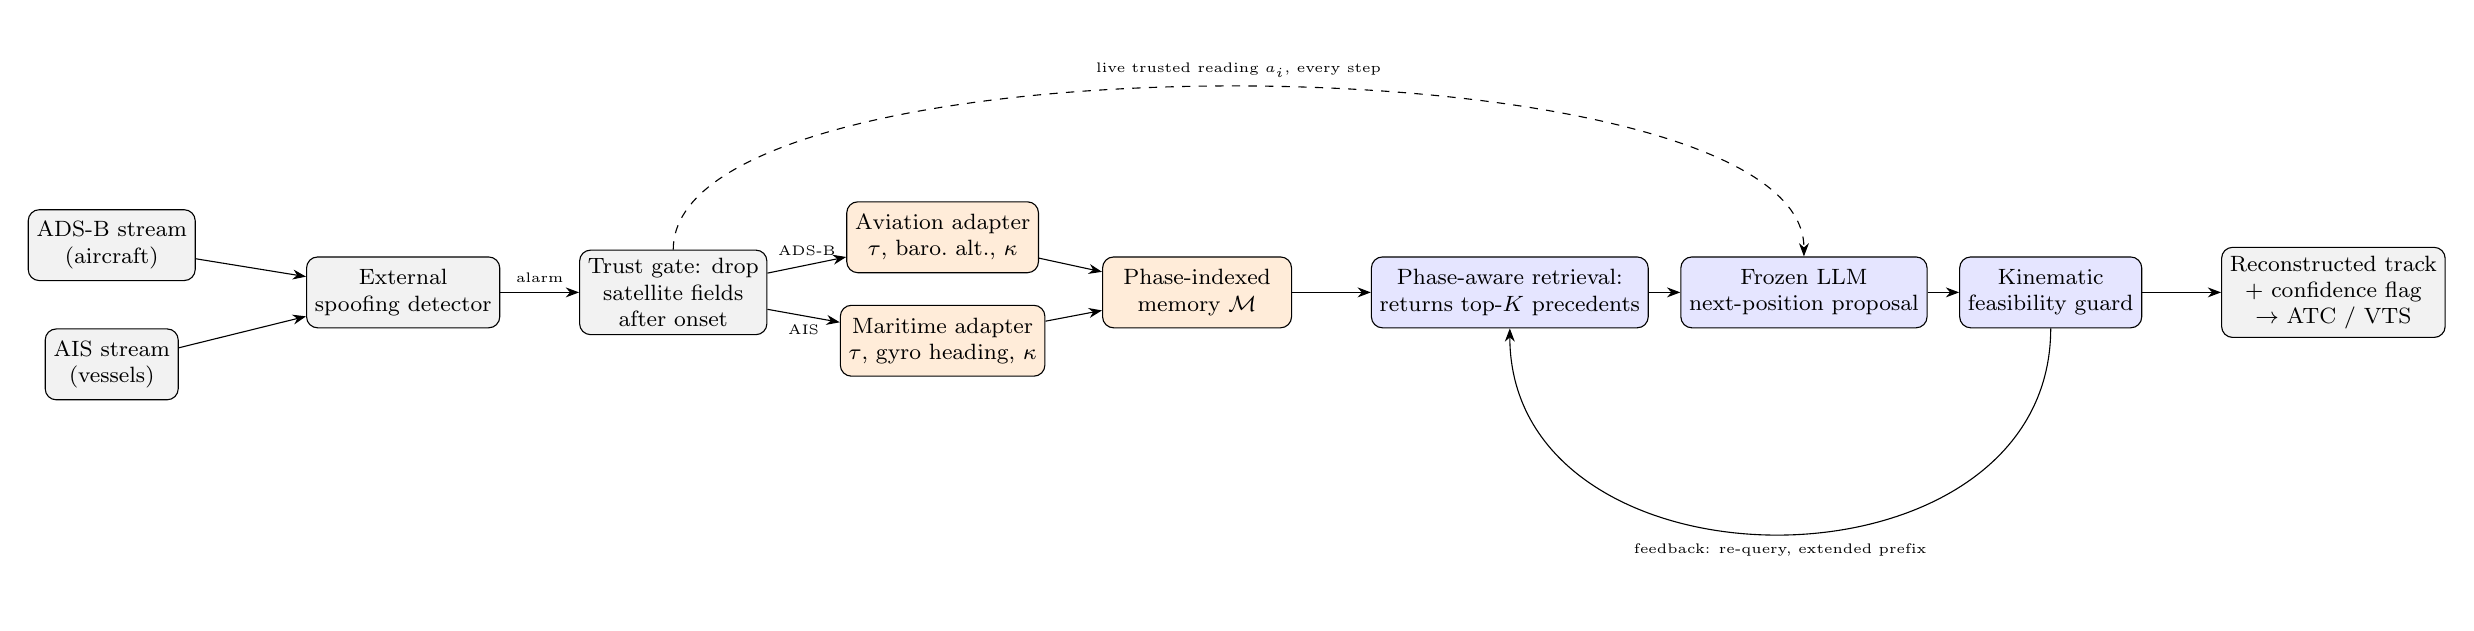
\begin{tikzpicture}[
  node distance=10mm and 8mm,
  box/.style={draw, rounded corners, align=center, minimum height=9mm, font=\footnotesize, inner sep=3pt},
  adapter/.style={box, fill=orange!15},
  engine/.style={box, fill=blue!10},
  io/.style={box, fill=gray!10},
  >=Stealth
]
\node[io] (adsb) {ADS-B stream\\(aircraft)};
\node[io, below=6mm of adsb] (ais) {AIS stream\\(vessels)};
\node[io, right=14mm of adsb, yshift=-6mm] (detector) {External\\spoofing detector};
\node[io, right=10mm of detector] (gate) {Trust gate: drop\\satellite fields\\after onset};
\node[adapter, right=10mm of gate, yshift=7mm] (adaptA) {Aviation adapter\\$\tau$, baro.\ alt., $\kappa$};
\node[adapter, below=4mm of adaptA] (adaptM) {Maritime adapter\\$\tau$, gyro heading, $\kappa$};
\node[adapter, right=8mm of adaptA, yshift=-7mm, minimum width=24mm] (memory) {Phase-indexed\\memory $\mathcal{M}$};
\node[engine, right=10mm of memory, minimum width=26mm] (retrieval) {Phase-aware retrieval:\\returns top-$K$ precedents};
\node[engine, right=4mm of retrieval] (llm) {Frozen LLM\\next-position proposal};
\node[engine, right=4mm of llm] (guard) {Kinematic\\feasibility guard};
\node[io, right=10mm of guard] (out) {Reconstructed track\\+ confidence flag\\$\to$ ATC / VTS};
\draw[->] (adsb) -- (detector);
\draw[->] (ais) -- (detector);
\draw[->] (detector) -- node[above,font=\tiny]{alarm} (gate);
\draw[->] (gate) -- node[above,font=\tiny]{ADS-B} (adaptA);
\draw[->] (gate) -- node[below,font=\tiny]{AIS} (adaptM);
\draw[->] (adaptA) -- (memory);
\draw[->] (adaptM) -- (memory);
\draw[->] (memory) -- (retrieval);
\draw[->] (retrieval) -- (llm);
\draw[->] (llm) -- (guard);
\draw[->] (guard) -- (out);
\draw[->] (guard.south) to[out=270,in=270,looseness=1.3] node[below,font=\tiny]{feedback: re-query, extended prefix} (retrieval.south);
\draw[->, dashed] (gate.north) to[out=90,in=90,looseness=0.5] node[above,font=\tiny]{live trusted reading $a_i$, every step} (llm.north);
\end{tikzpicture}%
}
\caption{Architecture of the real-time, domain-agnostic system. Both
surveillance streams pass through the same detector interface and trust
gate. A domain adapter (orange) supplies the domain-specific parts: the
textual-state prompt template, the trusted non-satellite signal, the
kinematic constants, and the phase-indexed memory $\mathcal{M}$ built from
that domain's history -- shown as a separate node from the shared engine's
retrieval step (blue), which searches $\mathcal{M}$ and returns only the
top-$K$ precedents for the current query, not the memory itself. The dashed
arrow shows the trusted reading $a_i$ (heading or barometric altitude)
entering the loop live at every step, independently of the one-shot
adapter routing above it. The engine asks a frozen large language model for
the next position and accepts it only inside the kinematic envelope; the
accepted position extends the verified prefix, and the query is rebuilt
from it before the next retrieval. ATC: air traffic control; VTS: vessel
traffic service.}
\label{fig:architecture}
\end{figure}

\section{Domain instantiations}
\label{sec:instantiation}

Table~\ref{tab:adapters} lists both adapters side by side.

\begin{table}[t]
\centering
\caption{Domain adapters used in this study. Everything outside this table
(embedding model, retrieval, prompting protocol, iterative loop, feasibility
guard and output schema) is shared code. The maritime column is new in this
paper.}
\label{tab:adapters}
\footnotesize
\begin{tabular}{p{3.0cm}p{4.0cm}p{4.0cm}}
\toprule
Adapter element & Aviation (ADS-B) & Maritime (AIS) \\
\midrule
State schema $\mathcal{S}$ & Latitude, longitude, ground speed, track, barometric altitude & Latitude, longitude, speed over ground (SOG), course over ground (COG), heading \\
Untrusted after onset & Latitude, longitude, ground speed, track & Latitude, longitude, SOG, COG \\
Trusted signal $a$ & Barometric altitude (pressure sensor) & Gyrocompass true heading \\
Phase taxonomy $\mathcal{P}$ & Takeoff / cruise / landing & Departure / transit / arrival \\
Verbaliser $\tau$ (prompt) & Flight-phase template (\ref{app:templates}) & Voyage-phase template (\ref{app:templates}) \\
Environment $\mathcal{E}$ & Meteomatics: wind aloft, turbulence indicators & Open-Meteo Marine: waves, swell, current, wind, sea-surface temperature \\
Memory $\mathcal{M}$ & FlightRadar24 history; one index per phase & NOAA Marine Cadastre history; one index per phase and corridor \\
Kinematics $\kappa$ & $\Delta t = 120$\,s; $\alpha = 1.2$ & $\Delta t = 300$\,s (resampled); $\alpha = 1.2$ (Section~\ref{sec:maritime-calibration}) \\
Reference-speed rule & Inferred from consecutive accepted reconstructed positions & Held at the last trusted SOG for the whole blackout (Section~\ref{sec:maritime-speedrule}) \\
LLM backbone & gpt-5.1 (frozen) & gpt-4.1 (frozen) \\
Retrieved neighbours $K$ & 5 & 6 \\
\bottomrule
\end{tabular}
\end{table}

\subsection{Aviation adapter}

The aviation adapter is that of the conference version
\citep{felendler2026trajrag} and is summarised here only for completeness.
The trusted signal is barometric altitude, which comes from the air-data
system rather than the GNSS receiver. Phases (takeoff, cruise, landing) are
assigned from altitude trends. The verbaliser describes the flight phase,
time since takeoff, altitude trend, heading and speed trend and the aligned
wind and turbulence indicators. During a blackout, ground speed and heading
are not read from ADS-B; they are inferred from consecutive accepted
reconstructed positions and used as the reference speed of
Eq.~\eqref{eq:guard}.

\subsection{Maritime adapter}
\label{sec:maritime-adapter}

\paragraph{Trusted signal} On commercial vessels, true heading is normally
supplied by a gyrocompass, which is independent of GNSS, whereas SOG and COG
are computed by the GNSS receiver. We therefore treat heading as the
maritime counterpart of barometric altitude, and SOG and COG as untrusted
after onset. Heading was present on 98--99\% of AIS reports in our corpus,
comparable to the availability of barometric altitude in ADS-B. Vessels
whose heading comes from a satellite compass break this independence
assumption. We return to this point in Section~\ref{sec:threats}.

\paragraph{Phases and memory} Voyages are segmented into departure (leaving
the berth and manoeuvring), transit (steady channel or approach passage) and
arrival (slowing and berthing). One index is built per phase and per
corridor, so the adapter's memory for a port is simply a small set of
indices built from that port's history. This segmentation is computed
offline from each completed voyage's full SOG trend, which is the practical
way to build phase-indexed memory from historical data; it is not an
implementation of the online phase-assignment rule $\pi$ of
Section~\ref{sec:framework}, which is restricted to trusted information
available up to the current step. At evaluation time, each benchmark
voyage's phase label is taken from this offline segmentation, so the
maritime instantiation evaluates reconstruction \emph{within} a known phase
rather than online phase identification; we return to this in
Section~\ref{sec:threats}.

\paragraph{Verbaliser} The voyage template mirrors the flight template but
uses maritime vocabulary and drivers. A representative departure state
reads: ``Vessel type: cargo. 15.0 minutes into the departure phase, the
vessel is tracking northeast through the Galveston Bay entrance channel,
heading 048\textdegree{} with course over ground 045\textdegree{} and speed
over ground 8.4 knots, gradually accelerating away from berth. Sea state is
moderate, with 0.6\,m wave height and a light following swell; a moderate
current of 0.9\,km/h runs with the vessel's heading, and a 12\,km/h wind
blows from the southeast. Motion has been steady, with no abrupt heading
change.'' The environmental provider attaches wave height, direction and
period, swell height, ocean-current speed and direction, sea-surface
temperature and 10\,m wind speed and direction from Open-Meteo Marine
\citep{openmeteo2025}. \ref{app:templates} gives both templates
verbatim, together with a fully worked maritime reconstruction step.

\paragraph{Sampling} Unlike ADS-B, AIS reporting is irregular: Class A
transponders change their rate with speed and navigational status, and
messages are lost to channel contention \citep{itu2014ais}. Rather than
letting the guard handle a variable $\Delta t$, the adapter resamples every
voyage onto a uniform 5-minute grid before segmentation. We verified that
all consecutive points within a segmented phase are exactly 300\,s apart.
This keeps the engine identical across domains, since the irregularity is
absorbed by the adapter's preprocessing.

\paragraph{Reference-speed rule}
\label{sec:maritime-speedrule}
The maritime $\mathrm{SPEEDRULE}$ holds the reference speed $v$ of
Eq.~\eqref{eq:guard} at the last \emph{trusted} SOG -- the value recorded
immediately before onset -- for the entire blackout, rather than updating it
from any post-onset field. This is the deployable rule used throughout
Section~\ref{sec:results}: it uses no information that a real blackout would
withhold. An earlier implementation instead updated the reference speed from
the recorded SOG at each reconstructed step; because SOG is GNSS-derived,
that variant used information a genuine blackout would not provide, and we
do not report it as a result in this paper. Section~\ref{sec:r1-result}
reports the corrected, deployable numbers together with the size of the
effect relative to that earlier, non-deployable variant, as a transparency
check rather than as an additional claimed result.

\section{Experimental design}
\label{sec:design}

\subsection{Data}
\label{sec:data}

Table~\ref{tab:datasets} summarises both corpora. The aviation corpus is
described in \citet{felendler2026trajrag}. The maritime corpus is new. We
downloaded 44 days of raw AIS position reports (19 April--1 June 2025, the
same calendar window as the aviation collection) from the NOAA Marine
Cadastre \citep{noaa2025marinecadastre}, a public United States government
archive with no access restrictions, which supports replication. Two
corridors with contrasting geometry were selected. The Houston Ship Channel,
from the Galveston Bay entrance to the Port of Houston, is a long, narrow
inland channel with dense tanker and cargo traffic. The Los Angeles/Long
Beach approach is a shorter, more open approach. From 26.2 million reports
we reconstructed 3,506 cargo and tanker voyages, segmented them into phases
and attached the marine environmental context. For testing we randomly
selected 250 vessels (125 per corridor) with at least four 5-minute points
in every phase, the same minimum segment length as in aviation; selection is
a uniform random sample over the full collection window, with no
chronological holdout by itself. AIS-ACNet's training and validation sets
exclude all test voyages and are themselves chronologically split
(Section~\ref{sec:baselines}).

An earlier implementation of TrajRAG's retrieval had two problems. First, it
excluded only the exact query voyage from a corridor's corpus-wide index,
not the other 124 test voyages, so a query could retrieve another test
voyage as a precedent -- retrieval memory contamination, not a disclosable
design choice. Second, the memory had no chronological cutoff, so a query
could retrieve a precedent recorded after it, which a real-time deployment
could never do. We rebuilt the memory to fix both: a corridor's retrieval
index is now built only from the chronologically earliest half of its
non-test voyages (1,141 of 2,283 non-test Houston voyages; 486 of 973
non-test Los Angeles/Long Beach voyages), and retrieval additionally
excludes every voyage in the test set, not only the query. Every TrajRAG
reconstruction reported in this paper queries only this pre-cutoff memory,
so no retrieved precedent can postdate the query, by construction rather
than by an exclusion list.

Reconstructing under the corrected memory, and under the corrected
preprocessing of Section~\ref{sec:preprocessing}, requires fresh LLM calls
for every query voyage, which this paper's budget could not extend to the
full 125-per-corridor test set together with the ablation and
matched-forecaster experiments of Sections~\ref{sec:maritime-ablations} and
\ref{sec:design} below. We therefore report TrajRAG's headline maritime
results on a smaller, still randomly-drawn common test set: 50 Houston and
10 Los Angeles/Long Beach voyages, sampled from the subset of the original
125-per-corridor test voyages that postdate each corridor's memory cutoff
(68 and 67 such voyages were available, respectively). Every other method
in Table~\ref{tab:extended} and Table~\ref{tab:corridor} -- Kalman, ARIMA,
LSTM, BiLSTM, Mean-Retrieval, Numeric-kNN and AIS-ACNet -- is rescored on
this identical 50/10-voyage set for a matched comparison; AIS-ACNet is
additionally reported on the full 125-voyage set as a robustness check that
the smaller matched sample is not anomalous (Section~\ref{sec:results}).
Section~\ref{sec:threats} discusses the resulting loss of statistical power,
particularly at Los Angeles/Long Beach.

\paragraph{Preprocessing correction}
\label{sec:preprocessing}
The 5-minute resampling grid originally interpolated latitude and longitude
with a time-weighted method that could use an AIS report recorded
\emph{after} a given grid timestamp, including the single most load-bearing
point in the whole pipeline: the last point of the verified prefix that
every method treats as ground truth to reconstruct from. Every other
resampled field (SOG, COG, heading, \ldots) already used a causal
last-observation-carried-forward rule; we moved latitude and longitude onto
the same rule, removing the leak. Rescoring the deterministic classical and
numeric baselines (Kalman, ARIMA, Numeric-kNN) on the corrected data versus
the original shows this is not a negligible effect: every one of 12
method/phase/corridor cells we checked became worse under the correction,
by 2--40\%, confirming the leak had been making reconstruction look easier
than it is. All results in this paper use the corrected data.

\begin{table}[t]
\centering
\caption{Datasets. The aviation corpus is the one used in the conference
version \citep{felendler2026trajrag}; the maritime corpus is new.}
\label{tab:datasets}
\footnotesize
\begin{tabular}{p{2.5cm}p{4.3cm}p{4.3cm}}
\toprule
 & Aviation & Maritime \\
\midrule
Source & FlightRadar24 ADS-B & NOAA Marine Cadastre AIS (public) \citep{noaa2025marinecadastre} \\
Corridors & Paris$\to$Rome; Barcelona$\to$Munich & Houston Ship Channel; Los Angeles/Long Beach approach \\
Collection window & 19 Apr--1 Jun 2025; 17 Dec 2025--18 Jan 2026 & 19 Apr--1 Jun 2025 (44 days) \\
Raw volume & 46,550 messages (Paris$\to$Rome) & 26.2 million position reports \\
Trajectories & 1,544 flights (931 + 613) & 3,506 voyages (2,408 Houston; 1,098 Los Angeles/Long Beach) \\
Sampling & $\approx$120\,s (native) & 300\,s (uniform resampling) \\
Test set & 100 flights, chronologically held out (Paris$\to$Rome) & 50 Houston + 10 Los Angeles/Long Beach vessels, each with $\geq 4$ points per phase, drawn from a 250-vessel (125 per corridor) pool and postdating the retrieval memory's chronological cutoff \\
Environmental context & Meteomatics & Open-Meteo Marine \citep{openmeteo2025} \\
\bottomrule
\end{tabular}
\end{table}

\subsection{Blackout protocol}

We simulate post-detection blackouts on real, uncorrupted trajectories, so
that the true positions are available as ground truth. Following a
safety-oriented, attack-agnostic stance, we model every attack (gradual
drift, velocity manipulation or capture-and-pull-off) the same way: all
satellite-derived fields after onset are withheld. In aviation, onset times
are randomised and blackouts last 5--15 steps (10--30\,min)
\citep{felendler2026trajrag}. In the maritime benchmark, each phase segment
of $N$ points is split at $\lfloor N/2 \rfloor$. The first half is the
verified prefix, and the second half is withheld and must be reconstructed.
This gives mean blackout durations of 37.2, 35.2 and 66.1\,min for
departure, transit and arrival on the Houston test set. The maritime
protocol is applied identically to every maritime method, including every
baseline: no baseline receives any field reported after the onset index.
Because the two domains use different protocols and sampling intervals,
absolute errors are compared within a domain, not across domains.

\subsection{Baselines}
\label{sec:baselines}

\textbf{Classical, recurrent and retrieval-only.} These are a Kalman filter
(a constant-velocity model that accounts for currents in the maritime case,
using only prefix data and environmental context), ARIMA fitted to each
verified prefix, LSTM and BiLSTM networks trained on the non-test voyages of
each phase (about 1,600--3,300 per phase), and Mean-Retrieval, which
averages the continuations of the top-$K$ retrieved segments without an
LLM.

\textbf{Numeric-kNN.} This baseline is a non-parametric retrieval model
operating on numbers rather than text. It finds the five training prefixes
of the same phase closest to the test prefix by mean point-wise Haversine
distance and predicts each withheld step as the coordinate-wise mean of
their continuations. It isolates the value of textual states combined with
LLM blending over plain numeric nearest neighbours.

\textbf{AIS-ACNet.} We retrain AIS-ACNet \citep{shin2024aisacnet} from its
public implementation on our voyages (on the corrected data of
Section~\ref{sec:preprocessing}), using a chronological 85/15
train/validation split of the non-test Houston voyages, and evaluate it on
the common test set with the same blackout boundary. We report it both on
the full 125-voyage test set and on the 50/10-voyage set TrajRAG is
evaluated on, to check that the smaller matched sample is not anomalous
(Section~\ref{sec:results}). AIS-ACNet's
convolutional receptive field is fixed, so we train one model per phase,
with the window set near the 95th percentile of the true half-phase length
(Table~\ref{tab:acnet-config}). Voyages whose true withheld half exceeds the
window are truncated to it for both the model's output and the scoring mask
-- 4, 6 and 5 of the 125 test voyages in departure, transit and arrival
respectively (3--5\% per phase); shorter ones are padded with edge values
and masked out of the loss and the metric. For the remaining 95--97\% of
voyages per phase, AIS-ACNet reconstructs exactly the same horizon as
TrajRAG; for the truncated tail, AIS-ACNet is scored only on the first
\emph{window} steps of the blackout, not the full one TrajRAG reconstructs.

\begin{table}[t]
\centering
\caption{Phase-specific AIS-ACNet configuration. The window is set near the
95th percentile of the true half-phase length so that most voyages are
predicted over their full withheld half.}
\label{tab:acnet-config}
\footnotesize
\begin{tabular}{lccc}
\toprule
Phase & Window (steps) & Residual blocks & Test voyages scored \\
\midrule
Departure & 21 & 7 & 125 \\
Transit & 15 & 5 & 125 \\
Arrival & 32 & 11 & 125 \\
\bottomrule
\end{tabular}
\end{table}

\textbf{Modern forecasters.} DLinear, PatchTST, iTransformer, Informer,
Autoformer, FEDformer and TimesNet are trained with the Time-Series-Library
implementations \citep{wu2023tslib} on eight features per step (latitude,
longitude, SOG, COG, heading, wave height, 10\,m wind speed and current
speed). The features are z-scored with training-split statistics.
Encoder--decoder models receive the tail of the \emph{observed} window as
their decoder warm-up, so no target value leaks into the input. These
architectures need fixed input and output lengths. Following the aviation
harness of the conference paper, we use a small exact-fit window per phase
(4, 3 and 4 steps for departure, transit and arrival) and include a voyage
only if its half-phase length matches the window. This retains about 80\%,
71\% and 77\% of eligible voyages. The forecasters therefore solve an
easier, shorter-horizon problem on a subset of voyages, and
Table~\ref{tab:extended} reports them in a separate block.

\subsection{Metrics and statistical testing}
\label{sec:metrics}

The primary metric is the mean Haversine error (MHE) \citep{zhao2024space}
over the withheld steps $T$,
\begin{equation}
\mathrm{MHE} = \frac{1}{|T|} \sum_{i \in T} d_{\mathrm{hav}}(\hat{y}_i, y_i),
\label{eq:mhe}
\end{equation}
reported per phase. A given absolute error means more for a slow ship than
for a fast one, so we also normalise MHE by two quantities that are
independent of the method and computed from ground truth: the mean distance
travelled during the blackout and the mean blackout duration. Differences
between TrajRAG and each full-horizon baseline are tested with paired
two-sided Wilcoxon signed-rank tests \citep{wilcoxon1945individual} on
per-voyage errors of the same voyages (50 Houston, 10 Los Angeles/Long
Beach). We report raw $p$-values and note
which conclusions survive a Bonferroni correction. We additionally report,
for each comparison, the median paired difference (baseline minus TrajRAG)
with a 95\% bootstrap confidence interval over 10,000 resamples of voyages,
and the median, 90th percentile and maximum of the per-voyage error
distribution for every full-horizon method.

\subsection{Implementation}
\label{sec:implementation}

Both instantiations use \texttt{text-embedding-3-large} as $g$ and FAISS
inner-product indices \citep{johnson2021billion}. The aviation adapter uses
\texttt{gpt-5.1} with $K=5$, the configuration selected in the conference
study. The maritime adapter uses \texttt{gpt-4.1} with $K=6$, fixed before
any maritime test-set result was observed; neither backbone was fine-tuned,
and no maritime hyperparameter was tuned on the test set. Per their
respective model documentation, \texttt{gpt-4.1}'s training data cutoff is
June 1, 2024 and \texttt{gpt-5.1}'s is September 30, 2024 -- both postdate
the Houston and LA/Long Beach voyage windows used in this study (19
April--1 June 2025 collection, but reflecting vessel traffic and port
operations that are not novel information the models could have memorised
verbatim). AIS-ACNet and the
seven forecasters are trained with Adam and early stopping (AIS-ACNet:
masked mean-squared error on position and auxiliary SOG/COG, patience 20, at
most 150 epochs; forecasters: mean-squared error, learning rate $10^{-3}$,
batch size 32, patience 15, at most 60 epochs). LLM decoding uses
temperature 0 for position generation and temperature 0.3 for the one-off
textual summary at blackout onset, in both domains.

\section{Results}
\label{sec:results}

All maritime TrajRAG numbers in this section use the deployable
\texttt{last\_trusted\_held} speed rule (Section~\ref{sec:maritime-speedrule})
and the corrected preprocessing and retrieval memory of
Sections~\ref{sec:preprocessing}--\ref{sec:data}. TrajRAG is evaluated on 50
Houston and 10 Los Angeles/Long Beach voyages; every other method in this
section is rescored on the identical set unless stated otherwise.

\subsection{Aviation reference point}
\label{sec:aviation-reference}

Table~\ref{tab:aviation-ref} condenses the aviation results of the conference
version into one row per baseline family. TrajRAG reduced mean error
relative to the best member of every family in every phase. The conference
study also reported four findings that frame the maritime experiments: (i)
removing retrieval caused the largest degradation in every phase; (ii)
replacing the LLM with neighbour averaging was significantly worse; (iii)
the feasibility guard mainly reduced variance and worst-case error; and (iv)
mixing several routes in one memory changed MHE by less than 1\,km. On four
real interference episodes with independent multilateration positions, the
reconstructions stayed within 8\,km of the reference on average
\citep{felendler2026trajrag}.

\begin{table}[t]
\centering
\caption{Aviation reference results, reproduced in condensed form from the
conference version \citep{felendler2026trajrag}: mean Haversine error (km)
of TrajRAG and of the best method in each baseline family, per flight phase
(100 held-out Paris$\to$Rome flights). The full per-method table,
ablations, backbone sensitivity and real-world case studies are reported
there.}
\label{tab:aviation-ref}
\footnotesize
\begin{tabular}{p{6.2cm}ccc}
\toprule
Method family (best member) & Takeoff & Cruise & Landing \\
\midrule
Classical: Kalman / ARIMA & 60.95 & 37.69 & 73.82 \\
Recurrent: LSTM / BiLSTM & 33.78 & 40.66 & 11.17 \\
Modern forecasters: DLinear / PatchTST / iTransformer & 43.99 & 19.79 & 35.47 \\
Retrieval only: Mean-Retrieval / Numeric-kNN & 48.94 & 30.80 & 8.52 \\
\textbf{TrajRAG (gpt-5.1)} & \textbf{20.78} & \textbf{9.84} & \textbf{2.46} \\
\bottomrule
\end{tabular}
\end{table}

\subsection{Transfer to shipping without training}

Table~\ref{tab:maritime-transfer} reports the maritime instantiation pooled
across both corridors (60 test vessels: 50 Houston, 10 Los Angeles/Long
Beach), deployable speed rule. With no model trained on maritime data,
TrajRAG has the lowest mean error of this baseline family in every phase.
It reduces error by a factor of 1.45 (departure) and 1.37 (transit) relative
to the Kalman filter, and 1.54 (arrival) relative to ARIMA, the strongest
baselines in those phases. The ranking of the baselines differs from
aviation: at sea, classical filters outperform recurrent networks and plain
retrieval, consistent with the more regular within-phase motion of large
vessels sampled every 5 minutes. TrajRAG remains first among these
baselines in both domains; Section~\ref{sec:extended-comparison} adds the
comparison against a trained, ship-specific network.

\begin{table}[t]
\centering
\caption{Maritime transfer: mean ($\mu$) and standard deviation ($\sigma$)
of the Haversine error (km) on 60 held-out vessels pooled across both
corridors (50 Houston, 10 Los Angeles/Long Beach; 180 phase-level
reconstructions). TrajRAG is used without any training on maritime data.}
\label{tab:maritime-transfer}
\footnotesize
\setlength{\tabcolsep}{4pt}
\begin{tabular}{lcccccc}
\toprule
\multirow{2}{*}{Method} & \multicolumn{2}{c}{Departure} & \multicolumn{2}{c}{Transit} & \multicolumn{2}{c}{Arrival} \\
\cmidrule(lr){2-3}\cmidrule(lr){4-5}\cmidrule(lr){6-7}
 & $\mu$ & $\sigma$ & $\mu$ & $\sigma$ & $\mu$ & $\sigma$ \\
\midrule
Kalman (current-aware constant velocity) & 2.84 & 2.26 & 2.62 & 3.80 & 3.58 & 4.19 \\
ARIMA & 3.29 & 2.38 & 3.65 & 3.90 & 1.95 & 2.77 \\
LSTM & 9.48 & 5.70 & 7.49 & 4.38 & 6.05 & 3.95 \\
BiLSTM & 8.93 & 4.80 & 12.22 & 7.30 & 15.07 & 19.18 \\
Mean-Retrieval & 12.52 & 11.91 & 7.95 & 6.36 & 6.55 & 5.25 \\
\textbf{TrajRAG} & \textbf{1.96} & \textbf{2.01} & \textbf{1.91} & \textbf{2.82} & \textbf{1.27} & \textbf{2.42} \\
\bottomrule
\end{tabular}
\end{table}

\subsection{Comparison with a trained ship-specific network and modern forecasters}
\label{sec:extended-comparison}

Table~\ref{tab:extended} and Fig.~\ref{fig:barplot} extend the comparison on
the common Houston test set (50 voyages), under the deployable speed rule.
Among full-horizon methods, two methods are far more accurate than the
rest: AIS-ACNet, which is trained on maritime data with one network per
phase, and TrajRAG, which is not trained on maritime data at all. Their
errors lie between 1.2 and 2.2\,km, while every other method lies between
1.9 and 16.4\,km. AIS-ACNet has a lower sample mean in all three phases
(1.80 vs.\ 2.19\,km departure, 1.66 vs.\ 1.95\,km transit, 1.18 vs.\
1.50\,km arrival), but Section~\ref{sec:significance} shows none of these
three gaps is statistically significant at $n=50$: a frozen-LLM,
retrieval-based reconstructor that sees no maritime training data at all is
statistically indistinguishable from a convolutional network purpose-built
and trained for this corridor. We read this as the relevant finding, not a
loss -- AIS-ACNet is among the strongest published ship-specific
trajectory networks, and matching it without any maritime training is the
comparison TrajRAG needs to win to be useful as a drop-in, training-free
alternative.

Numeric-kNN, which uses the same retrieval idea on raw coordinates, has 2.0
to 2.5 times the error of TrajRAG. Mean-Retrieval, which averages the
textually retrieved neighbours without an LLM, is worse than Numeric-kNN.
This compares the complete TrajRAG pipeline against two retrieval-only
baselines, not a single isolated component: Numeric-kNN differs from
TrajRAG in the retrieval representation (numeric vs.\ textual), the
combination rule (averaging vs.\ LLM generation) and access to live trusted
heading, so the gap cannot be attributed to the LLM alone. The no-retrieval
ablation of Section~\ref{sec:maritime-ablations} isolates retrieval's
contribution within the TrajRAG pipeline specifically, which matches the
qualitative pattern of the aviation ablation \citep{felendler2026trajrag}.

The short-window forecasters reach errors between 0.69 and 3.5\,km. On the
3-step transit window, several of them have lower values than TrajRAG has
over the full transit half-phase. This is expected: errors grow with
horizon, and these models are scored only on the first 3--4 steps of the
subset of voyages that fit their window. The block is included to document
that modern forecasters were evaluated, not to rank them against full-horizon
reconstruction.

To give the forecasters a genuine same-timestamps comparison rather than
only this caveat, we additionally reconstructed TrajRAG and re-scored
AIS-ACNet on the forecasters' own exact voyage subset and horizon (window
steps of 4, 3 and 4; $n=63$, 63 and 53 after also requiring the voyage to
postdate the retrieval memory's cutoff, Section~\ref{sec:data}).
Table~\ref{tab:item4-matched} reports the result: TrajRAG is more accurate
than AIS-ACNet on this short horizon in all three phases (1.30 vs.\
1.64\,km departure, 0.73 vs.\ 1.19\,km transit, 0.68 vs.\ 1.10\,km arrival).
Short-horizon reconstruction is close to a regime where the guard rarely
needs to bind and the retrieved precedent's early trajectory is highly
informative, which may explain why TrajRAG's relative advantage over
AIS-ACNet is clearer here than over the full withheld half (Table~\ref{tab:extended}).
A paired Wilcoxon test (Section~\ref{sec:significance}) confirms this
advantage is significant in all three phases.

The transit-phase values of TrajRAG (0.73) and iTransformer (0.734,
Table~\ref{tab:extended}) round to the same two decimals, leaving their
ordering unclear at that precision. Recomputed to full precision from the
saved per-step predictions, TrajRAG's matched-subset mean is
0.730561\,km (0.731 at three decimals) against iTransformer's
0.734297\,km: TrajRAG is lower. This is a precision clarification, not an
additional paired test -- the two means are still computed on different,
non-overlapping voyage subsets (TrajRAG's matched $n=63$ vs.\
iTransformer's own $n=118$ test split), so no significance claim is made
for this particular pair.

\begin{table}[t]
\centering
\caption{Matched short-window comparison: TrajRAG and AIS-ACNet scored on
the identical voyages and horizon as the modern forecasters of
Table~\ref{tab:extended}'s lower block (window steps in parentheses).
Mean Haversine error (km), Houston.}
\label{tab:item4-matched}
\footnotesize
\begin{tabular}{lccc}
\toprule
Method & Departure (4) & Transit (3) & Arrival (4) \\
\midrule
$n$ & 63 & 63 & 53 \\
AIS-ACNet & 1.64 & 1.19 & 1.10 \\
\textbf{TrajRAG} & \textbf{1.30} & \textbf{0.73} & \textbf{0.68} \\
\bottomrule
\end{tabular}
\end{table}

\begin{table}[t]
\centering
\caption{Extended maritime comparison on the common 50-voyage Houston Ship
Channel test set: mean Haversine error (km), deployable speed rule. Upper
block: methods that reconstruct the full withheld half of each phase,
scored on all 50 voyages per phase. AIS-ACNet's full-125-voyage-test-set
mean is 1.70 / 1.41 / 1.14 (departure/transit/arrival), close to its
50-voyage figure below, confirming the smaller matched sample is not
anomalous. Lower block: fixed-window forecasters that predict only a short,
exact-fit horizon on a smaller subset of voyages that fit the window
exactly ($n=113$, 118 and 99 for departure, transit and arrival); they are
not directly comparable with the upper block (Section~\ref{sec:baselines}) --
Table~\ref{tab:item4-matched} gives TrajRAG and AIS-ACNet on this same
subset and horizon. ``Training'' column: whether parameters are fitted on
maritime trajectories.}
\label{tab:extended}
\footnotesize
\setlength{\tabcolsep}{4pt}
\begin{tabular}{lcccc}
\toprule
Method & Maritime training & Departure & Transit & Arrival \\
\midrule
\multicolumn{5}{l}{\emph{Full-horizon reconstruction}} \\
Kalman & no & 3.164 & 2.614 & 4.229 \\
ARIMA & per voyage fit & 3.638 & 3.780 & 2.242 \\
LSTM & yes & 10.435 & 7.985 & 6.415 \\
BiLSTM & yes & 10.025 & 14.104 & 16.427 \\
Mean-Retrieval & no & 13.892 & 8.758 & 7.028 \\
Numeric-kNN & no & 5.534 & 3.928 & 3.171 \\
AIS-ACNet \citep{shin2024aisacnet} & yes (3 models) & \textbf{1.802} & \textbf{1.660} & \textbf{1.181} \\
TrajRAG (deployable rule) & no & 2.185 & 1.947 & 1.496 \\
\midrule
\multicolumn{5}{l}{\emph{Short exact-fit window (departure 4, transit 3, arrival 4 steps)}} \\
DLinear & yes & 3.529 & 3.081 & 3.259 \\
PatchTST & yes & 2.666 & 1.277 & 1.334 \\
iTransformer & yes & 2.405 & 0.734 & 1.214 \\
Informer & yes & 1.721 & 0.816 & 1.990 \\
Autoformer & yes & 2.076 & 0.693 & 1.667 \\
FEDformer & yes & 1.832 & 0.891 & 1.064 \\
TimesNet & yes & 1.449 & 0.759 & 0.624 \\
\bottomrule
\end{tabular}
\end{table}

\begin{figure}[t]
\centering
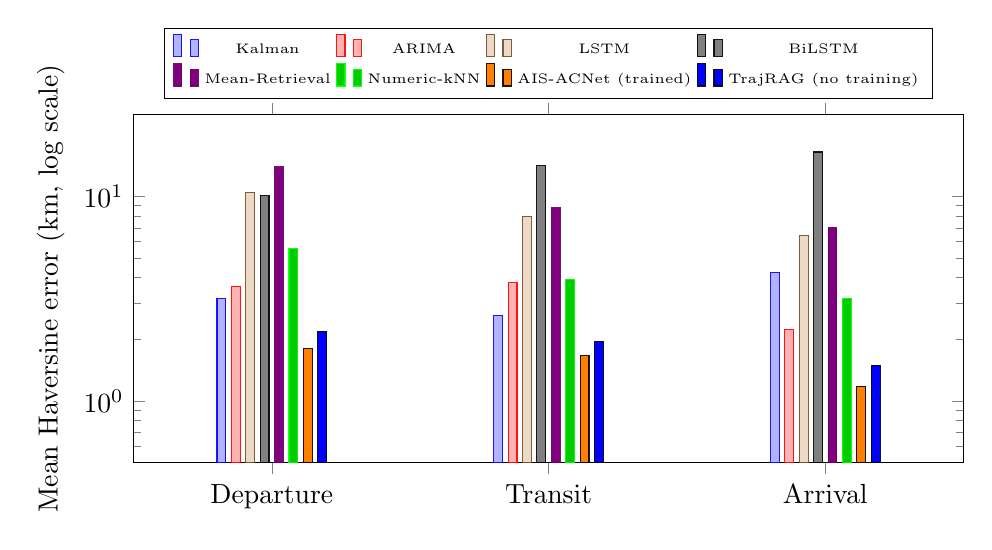
\begin{tikzpicture}
\begin{axis}[
  ybar, width=\linewidth, height=6cm,
  ymode=log, log origin=infty,
  symbolic x coords={Departure,Transit,Arrival},
  xtick=data, bar width=3.2pt,
  ylabel={Mean Haversine error (km, log scale)},
  legend style={font=\tiny, at={(0.5,1.25)}, anchor=north, legend columns=4},
  enlarge x limits=0.25, ymin=0.5, ymax=25,
  nodes near coords=, every axis plot/.append style={draw opacity=0.9},
]
\addplot coordinates {(Departure,3.164) (Transit,2.614) (Arrival,4.229)};
\addplot coordinates {(Departure,3.638) (Transit,3.780) (Arrival,2.242)};
\addplot coordinates {(Departure,10.435) (Transit,7.985) (Arrival,6.415)};
\addplot coordinates {(Departure,10.025) (Transit,14.104) (Arrival,16.427)};
\addplot coordinates {(Departure,13.892) (Transit,8.758) (Arrival,7.028)};
\addplot coordinates {(Departure,5.534) (Transit,3.928) (Arrival,3.171)};
\addplot[fill=orange] coordinates {(Departure,1.802) (Transit,1.660) (Arrival,1.181)};
\addplot[fill=blue] coordinates {(Departure,2.185) (Transit,1.947) (Arrival,1.496)};
\legend{Kalman,ARIMA,LSTM,BiLSTM,Mean-Retrieval,Numeric-kNN,AIS-ACNet (trained),TrajRAG (no training)}
\end{axis}
\end{tikzpicture}
\caption{Full-horizon maritime reconstruction error on the common 50-voyage
Houston Ship Channel test set (values from Table~\ref{tab:extended},
deployable speed rule). TrajRAG and the trained AIS-ACNet network form a
separate accuracy tier from all other methods. TrajRAG reaches this tier
without any training on maritime trajectories.}
\label{fig:barplot}
\end{figure}

\subsection{Two simple kinematic baselines: holding position and dead reckoning on trusted heading}
\label{sec:simple-baselines}

Two further baselines, neither requiring training or an LLM call, isolate
how much of the above comparisons could be explained by the simplest
possible use of the trusted signals alone. \emph{Constant position} predicts
that the vessel remains at its last trusted position for the entire
blackout. \emph{Heading dead reckoning (heading DR)} starts from the last
trusted position, holds the last trusted SOG fixed for the whole blackout
(the same convention as TrajRAG's deployable speed rule,
Section~\ref{sec:maritime-speedrule}), reads the live trusted heading
available at each reconstruction step, and propagates position step by step
with the geographic destination-point formula (not a planar addition of
kilometres to latitude/longitude), using only arithmetic on the corrected
voyage data -- no model of any kind. Both are evaluated on the identical
main-set voyages and timestamps as Table~\ref{tab:extended}.

\begin{table}[t]
\centering
\caption{Two training-free kinematic baselines, mean Haversine error (km),
evaluated on the same 50 Houston and 10 Los Angeles/Long Beach voyages as
Table~\ref{tab:extended}. \emph{Constant position}: holds the last trusted
position fixed. \emph{Heading DR}: dead reckoning from the last trusted
position using the last trusted SOG (held fixed) and the live trusted
heading at each step.}
\label{tab:simple-baselines}
\footnotesize
\setlength{\tabcolsep}{4pt}
\begin{tabular}{lcccccc}
\toprule
\multirow{2}{*}{Method} & \multicolumn{3}{c}{Houston Ship Channel} & \multicolumn{3}{c}{LA / Long Beach} \\
\cmidrule(lr){2-4}\cmidrule(lr){5-7}
 & Dep. & Trans. & Arr. & Dep. & Trans. & Arr. \\
\midrule
Constant position & 5.627 & 7.914 & 2.759 & 2.648 & 3.933 & 0.492 \\
Heading DR & 1.437 & 1.378 & 2.447 & 0.823 & 1.523 & 0.142 \\
AIS-ACNet (trained) & 1.802 & 1.660 & 1.181 & 1.128 & 1.947 & 1.020 \\
TrajRAG (no training) & 2.185 & 1.947 & 1.496 & 0.811 & 1.712 & 0.111 \\
\bottomrule
\end{tabular}
\end{table}

Constant position is a weak baseline everywhere except Los Angeles/Long
Beach arrival, where many vessels are nearly stationary while berthing: it
reaches 0.492\,km there, deceptively close to the other methods'
range. Even so, TrajRAG (0.111\,km) and heading DR itself (0.142\,km) both
still beat it by a factor of 3--4, so TrajRAG's low Los Angeles/Long Beach
arrival error is not mainly an artefact of recognising that the vessel is
not moving; genuine residual motion is being captured.

Heading DR is a far stronger baseline than its two parameters suggest. It
is more accurate than \emph{both} TrajRAG and the trained AIS-ACNet network
in Houston departure and transit and in Los Angeles/Long Beach transit, and
close to TrajRAG in the other two departure/arrival cells. It is clearly
worse than both in Houston arrival (2.447 vs.\ 1.496 and 1.181\,km), the
one phase dominated by a sustained turning manoeuvre into berth. Read
together with the non-significant no-heading ablation of
Section~\ref{sec:maritime-ablations}, this suggests that live trusted
heading alone already carries most of the usable signal in straight,
steady-speed phases, for any downstream method that consumes it -- which is
also why TrajRAG's own sensitivity to heading access, isolated from
everything else in its pipeline, is hard to detect at this sample size. The
harder, more differentiating comparisons for every method are concentrated
in manoeuvre-heavy phases such as arrival, not in departure or transit.

This result does not make heading DR a credible operational substitute,
for reasons intrinsic to the method rather than to this particular
evaluation. (i) It propagates a straight chord along the single most
recently reported heading for the whole inter-report interval, so a
sustained turn accumulates geometric error regardless of how often heading
is sampled -- exactly the arrival-phase degradation observed above, since
heading describes where the bow points at an instant, not the curved path
the vessel traces while turning, and can further diverge from the true
course over ground under current-induced leeway or set, which this method
has no way to represent. (ii) It has no error-correcting mechanism: once a
single noisy heading or SOG reading is propagated, nothing re-anchors the
estimate to a plausible position for the rest of the blackout, whereas
TrajRAG's guard and retrieved precedent re-ground the trajectory at every
step. (iii) It carries no spatial context -- no awareness of the fairway,
traffic separation scheme, charted obstructions or other vessels -- so
nothing prevents it from projecting a track across a jetty or shoal if the
reported heading does not track the channel's curvature. (iv) It can only
assume the present course continues; it has no model of \emph{when} a
vessel is likely to turn, so it structurally cannot anticipate the one
class of event -- a course change -- that reconstruction during a blackout
is most needed to recover, unlike TrajRAG's retrieved precedents, which
encode the actual historical turn geometry for the corridor and phase. (v)
Its competitiveness here is likely corridor- and vessel-class-specific:
large commercial vessels transiting dredged, largely straight channels at
steady speed are an easy case for any method that merely continues the
current heading, and the same assumption would be expected to fail in
congested or small-craft traffic, which neither corridor in this paper
tests. (vi) It depends on exactly the same trusted-signal assumption
already flagged as a threat to validity (Section~\ref{sec:threats}, item
v): a genuinely GNSS-independent heading sensor. A vessel without one
leaves this baseline with nothing to fall back on, whereas TrajRAG degrades
more gracefully, since removing live heading access does not significantly
change its own accuracy.

\subsection{Distribution of per-voyage error}
\label{sec:distribution}

Table~\ref{tab:distribution} reports the median, 90th percentile and
maximum per-voyage error for every full-horizon method under the deployable
rule. TrajRAG has a heavier tail than AIS-ACNet in every phase despite a
comparable median: departure (max 10.24\,km vs.\ 8.28\,km; median 1.25 vs.\
1.45\,km), transit (max 16.72\,km vs.\ 12.88\,km; median 0.92 vs.\
0.79\,km) and arrival (max 16.78\,km vs.\ 13.60\,km; median 0.89 vs.\
0.76\,km). This heavy tail is consistent with the non-significant
differences in Section~\ref{sec:significance}: the mean gap between the two
methods in every phase is driven by a minority of TrajRAG voyages with
large errors rather than by a consistent per-voyage advantage for either
method.

\begin{table}[t]
\centering
\caption{Distribution of per-voyage Haversine error (km), full-horizon
methods, 50 Houston Ship Channel test voyages, deployable speed rule for
TrajRAG.}
\label{tab:distribution}
\footnotesize
\setlength{\tabcolsep}{3pt}
\begin{tabular}{lcccccccccccc}
\toprule
\multirow{2}{*}{Method} & \multicolumn{3}{c}{Departure} & \multicolumn{3}{c}{Transit} & \multicolumn{3}{c}{Arrival} \\
\cmidrule(lr){2-4}\cmidrule(lr){5-7}\cmidrule(lr){8-10}
 & med. & p90 & max & med. & p90 & max & med. & p90 & max \\
\midrule
Kalman       & 2.51 & 5.81  & 11.66 & 1.19 & 7.88  & 20.39 & 2.14 & 10.70 & 17.37 \\
ARIMA        & 2.56 & 6.53  & 9.74  & 2.60 & 7.30  & 20.40 & 1.37 & 4.62  & 17.37 \\
LSTM         & 10.16 & 16.86 & 27.05 & 6.68 & 14.15 & 18.66 & 6.02 & 13.21 & 15.91 \\
BiLSTM       & 9.31 & 15.37 & 21.41 & 14.41 & 21.62 & 28.66 & 6.22 & 54.99 & 63.17 \\
Mean-Retrieval & 7.70 & 29.77 & 52.18 & 7.35 & 16.95 & 34.45 & 5.79 & 12.53 & 26.48 \\
Numeric-kNN  & 4.59 & 10.46 & 20.29 & 1.92 & 7.66  & 32.27 & 0.92 & 7.68  & 28.36 \\
AIS-ACNet    & 1.45 & 2.92  & 8.28  & 0.79 & 2.94  & 12.88 & 0.76 & 2.05  & 13.60 \\
TrajRAG      & 1.25 & 5.03  & 10.24 & 0.92 & 3.73  & 16.72 & 0.89 & 3.47  & 16.78 \\
\bottomrule
\end{tabular}
\end{table}

\subsection{Normalised error}

Table~\ref{tab:normalized} rescales the full-horizon errors by distance
travelled and by blackout duration. Arrival is the slowest phase: ships
cover only 3.18\,km on average during a 70-minute blackout. A small absolute
error is therefore a large relative one. The Kalman filter's arrival error,
for example, exceeds the distance the ship actually travelled (ratio 1.33),
which means that simply predicting no movement would have done better.
Under both normalisations TrajRAG and AIS-ACNet remain the two best methods
in every phase. TrajRAG's transit error is about 15.7\% of the distance
travelled.

\begin{table}[t]
\centering
\caption{Normalised error for the full-horizon methods (50 Houston Ship
Channel voyages, deployable speed rule for TrajRAG). ``/dist'': mean error
divided by the mean true distance travelled during the blackout
(dimensionless). ``/min'': mean error divided by the mean blackout duration
(km\,min$^{-1}$). Mean distance travelled: 9.19\,km (departure), 12.38\,km
(transit), 3.18\,km (arrival); mean blackout duration: 31.8, 36.7 and
69.9\,min. Best value per column in bold.}
\label{tab:normalized}
\footnotesize
\setlength{\tabcolsep}{4pt}
\begin{tabular}{lcccccc}
\toprule
\multirow{2}{*}{Method} & \multicolumn{2}{c}{Departure} & \multicolumn{2}{c}{Transit} & \multicolumn{2}{c}{Arrival} \\
\cmidrule(lr){2-3}\cmidrule(lr){4-5}\cmidrule(lr){6-7}
 & /dist & /min & /dist & /min & /dist & /min \\
\midrule
Kalman & 0.344 & 0.100 & 0.211 & 0.071 & 1.330 & 0.060 \\
ARIMA & 0.396 & 0.114 & 0.305 & 0.103 & 0.705 & 0.032 \\
LSTM & 1.136 & 0.328 & 0.645 & 0.218 & 2.017 & 0.092 \\
BiLSTM & 1.091 & 0.315 & 1.139 & 0.384 & 5.166 & 0.235 \\
Mean-Retrieval & 1.512 & 0.437 & 0.707 & 0.239 & 2.210 & 0.101 \\
Numeric-kNN & 0.602 & 0.174 & 0.317 & 0.107 & 0.997 & 0.045 \\
AIS-ACNet & \textbf{0.196} & \textbf{0.057} & \textbf{0.134} & \textbf{0.045} & \textbf{0.371} & \textbf{0.017} \\
TrajRAG & 0.238 & 0.069 & 0.157 & 0.053 & 0.470 & 0.021 \\
\bottomrule
\end{tabular}
\end{table}

\subsection{Statistical significance}
\label{sec:significance}

Testing many comparisons inflates the chance of an apparently significant
result by chance, and a non-significant result on its own does not
establish that two methods are equivalent. We therefore pre-register four
families of related comparisons and apply Holm's step-down correction
(family-wise $\alpha = 0.05$) within each: (F1) Houston main set, TrajRAG
vs.\ seven methods $\times$ three phases (21 tests, this subsection); (F2)
Los Angeles/Long Beach main set, TrajRAG vs.\ six methods $\times$ three
phases (18 tests, Table~\ref{tab:wilcoxon-la}); (F3) the short-horizon
matched comparison, TrajRAG vs.\ AIS-ACNet $\times$ three phases (3 tests,
Table~\ref{tab:item4-wilcoxon}); and (F4) the maritime ablations, three
configurations $\times$ three phases (9 tests,
Section~\ref{sec:maritime-ablations}). Corrections are applied within each
family, not pooled across families, since each answers a different
scientific question. iTransformer and the other modern forecasters are
excluded from every family: only their aggregate error was saved, over a
voyage subset that does not match TrajRAG's, so no paired test against them
is possible from saved outputs (Section~\ref{sec:threats}).

Table~\ref{tab:wilcoxon} gives paired Wilcoxon tests, deployable speed rule,
$n=50$, with both the raw and the Holm-corrected $p$-value. TrajRAG is
significantly more accurate than the Kalman filter, ARIMA, LSTM, BiLSTM,
Mean-Retrieval and Numeric-kNN in all three phases, surviving Holm
correction within this 21-test family ($p_{\text{Holm}} \leq 2.5 \times
10^{-2}$). Against AIS-ACNet, TrajRAG is not statistically distinguishable
from it in any of the three phases ($p = 0.77$, $0.56$ and $0.50$ for
departure, transit and arrival respectively), despite AIS-ACNet's lower
sample mean in all three. Pooling both corridors (Houston's 50 voyages and
Los Angeles/Long Beach's 10, $n=60$) for additional power does not change
this: $p=0.83$, $0.80$ and $0.52$. Given AIS-ACNet is trained specifically
for this task and TrajRAG uses no maritime training data at all, we read
this as TrajRAG matching a strong, purpose-built baseline rather than as a
weak result -- though, per the caveat above, a non-significant difference
is not evidence that the two methods are equivalent, only that this sample
does not resolve a difference.

Table~\ref{tab:bootstrap} reports the median paired difference (baseline
minus TrajRAG) with a 95\% bootstrap confidence interval. Every interval for
AIS-ACNet includes zero (departure $[-0.35, 0.30]$, transit $[-0.31, 0.23]$,
arrival $[-0.37, 0.38]$\,km), consistent with the non-significant Wilcoxon
results in all three phases. Every interval against every other baseline
excludes zero and is entirely positive, consistent with TrajRAG's
significant advantage over all of them. Fig.~\ref{fig:forest-houston}
plots the corresponding \emph{mean}, rather than median, paired difference
with its own 95\% bootstrap confidence interval (10,000 resamples of
voyage identities, not of individual trajectory points), for the same 21
comparisons, Holm-corrected within this family: the qualitative picture is
identical to Table~\ref{tab:bootstrap}, with only the three AIS-ACNet
intervals straddling zero.

\begin{figure}[t]
\centering
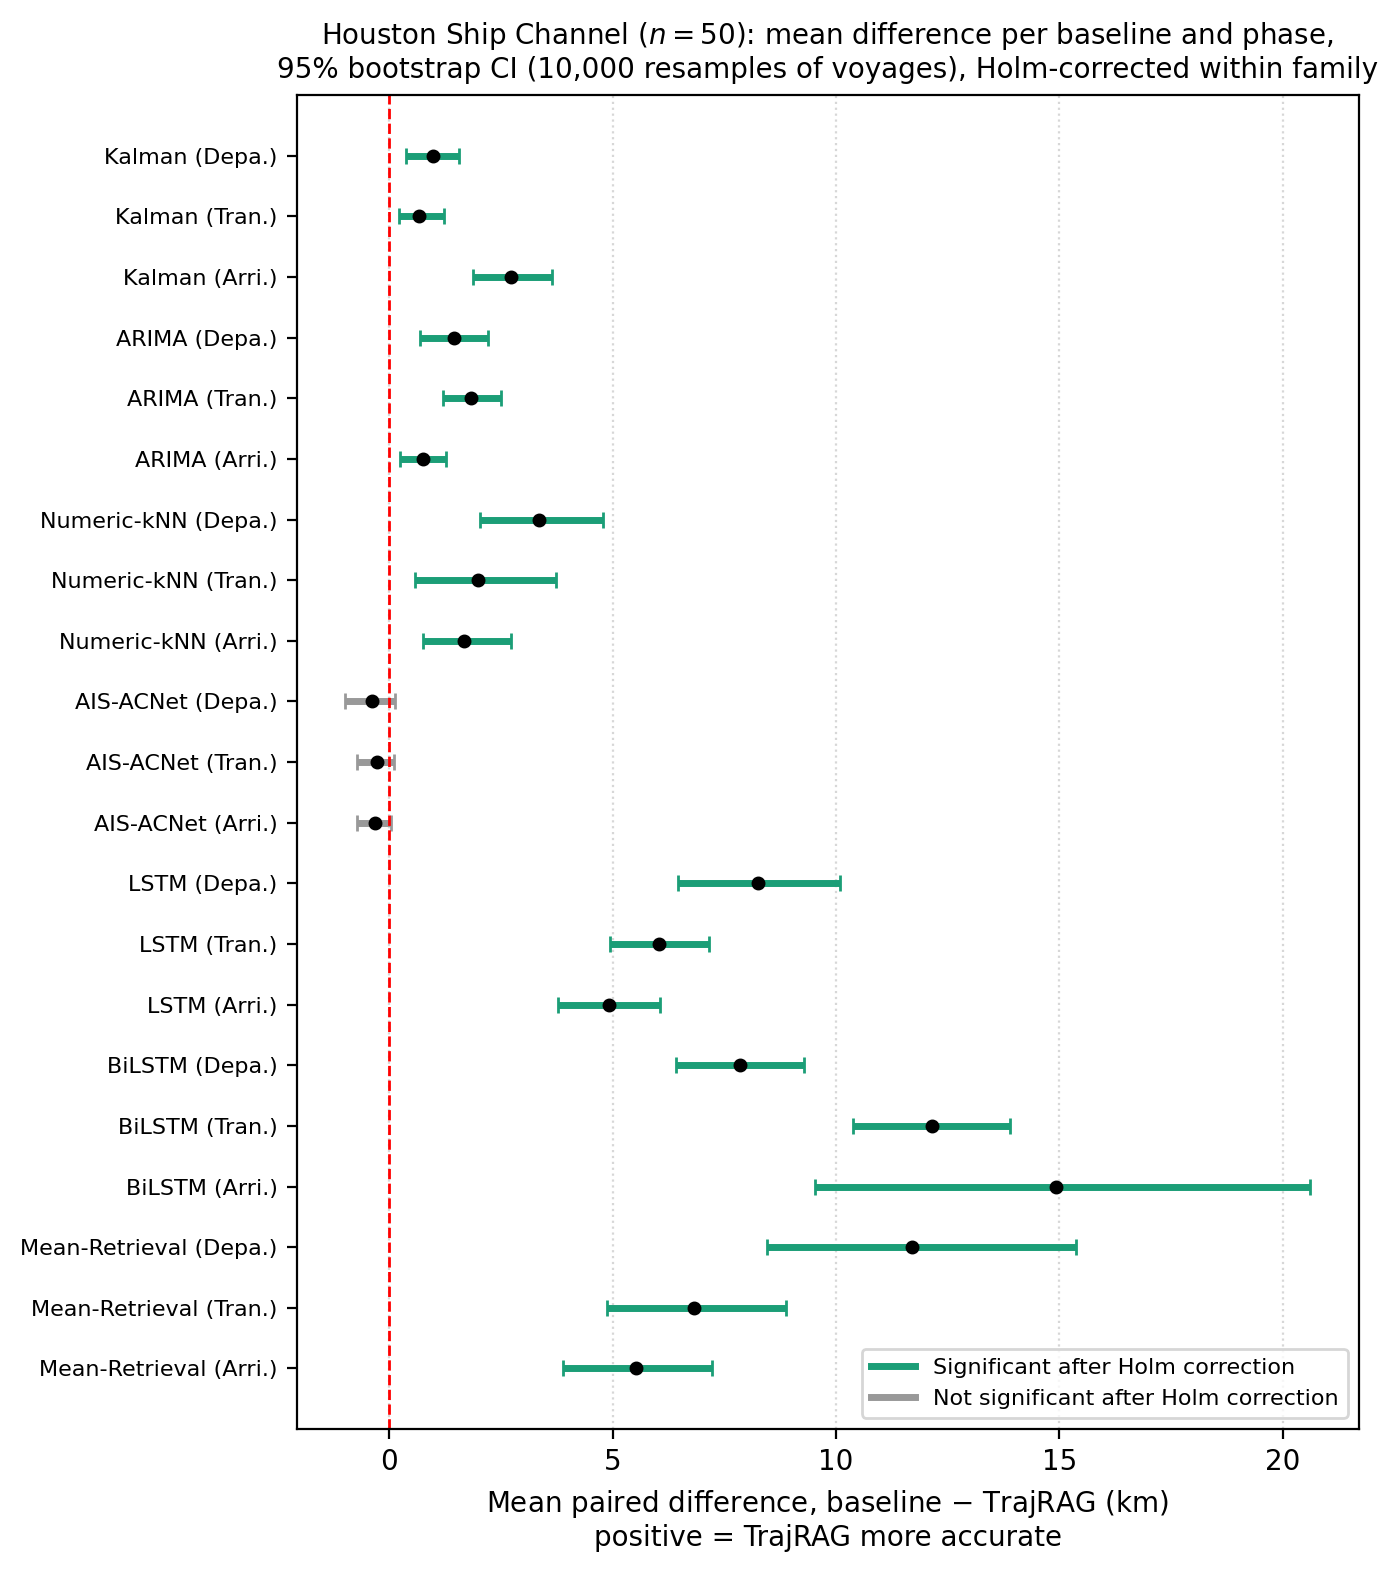
\includegraphics[width=\linewidth]{figures/forest_plot_houston_main.png}
\caption{Mean paired difference (baseline $-$ TrajRAG, km; positive =
TrajRAG more accurate) with 95\% bootstrap confidence interval (10,000
resamples of voyage identities), Houston Ship Channel, $n=50$, deployable
speed rule. Green: significant after Holm correction within this 21-test
family; grey: not significant. This figure reports the mean difference and
its uncertainty; Table~\ref{tab:bootstrap} reports the corresponding
median-difference interval and Table~\ref{tab:extended} the exact mean
errors themselves.}
\label{fig:forest-houston}
\end{figure}

\begin{table}[t]
\centering
\caption{Paired two-sided Wilcoxon signed-rank tests, TrajRAG vs.\ each
method, Los Angeles/Long Beach ($n=10$). $p_{\text{Holm}}$: Holm-corrected
within the 18-test family of this corridor. Bold: not significant at the
0.05 level after correction. Numeric-kNN was never rescored for this
corridor (Section~\ref{sec:threats}) and is omitted, not invented.}
\label{tab:wilcoxon-la}
\footnotesize
\setlength{\tabcolsep}{3pt}
\begin{tabular}{lcccccc}
\toprule
\multirow{2}{*}{TrajRAG vs.} & \multicolumn{2}{c}{Departure} & \multicolumn{2}{c}{Transit} & \multicolumn{2}{c}{Arrival} \\
\cmidrule(lr){2-3}\cmidrule(lr){4-5}\cmidrule(lr){6-7}
 & $p$ & $p_{\text{Holm}}$ & $p$ & $p_{\text{Holm}}$ & $p$ & $p_{\text{Holm}}$ \\
\midrule
Kalman & 0.049 & \textbf{0.342} & 0.049 & \textbf{0.342} & 0.014 & \textbf{0.123} \\
ARIMA & 0.049 & \textbf{0.342} & 0.010 & \textbf{0.098} & 0.232 & \textbf{0.697} \\
LSTM & $2.0 \times 10^{-3}$ & $0.035$ & $2.0 \times 10^{-3}$ & $0.035$ & $2.0 \times 10^{-3}$ & $0.035$ \\
BiLSTM & $2.0 \times 10^{-3}$ & $0.035$ & 0.131 & \textbf{0.523} & $2.0 \times 10^{-3}$ & $0.035$ \\
Mean-Retrieval & $2.0 \times 10^{-3}$ & $0.035$ & 0.014 & \textbf{0.123} & $2.0 \times 10^{-3}$ & $0.035$ \\
AIS-ACNet & 0.275 & \textbf{0.697} & 0.432 & \textbf{0.697} & $2.0 \times 10^{-3}$ & $0.035$ \\
\bottomrule
\end{tabular}
\end{table}

At $n=10$, four of the six raw $p$-values below 0.05 (every Kalman cell and
departure ARIMA) no longer survive Holm correction within this 18-test
family; only LSTM, BiLSTM and Mean-Retrieval remain significant in most
phases, and AIS-ACNet only in arrival (where TrajRAG's 0.111\,km mean is
far below AIS-ACNet's 1.020\,km, Table~\ref{tab:corridor}). This is
consistent with, and sharpens, the existing caution that the $n=10$ cell
size is underpowered (Section~\ref{sec:threats}): it does not mean the two
corridors behave differently, only that fewer voyages give less power to
confirm a Houston-scale effect at Los Angeles/Long Beach once correctly
accounting for testing six baselines across three phases.

\begin{table}[t]
\centering
\caption{Paired two-sided Wilcoxon signed-rank test, TrajRAG vs.\
AIS-ACNet, short-horizon matched subset (Table~\ref{tab:item4-matched}).
$p_{\text{Holm}}$: Holm-corrected within this 3-test family.}
\label{tab:item4-wilcoxon}
\footnotesize
\begin{tabular}{lccc}
\toprule
 & Departure ($n=63$) & Transit ($n=63$) & Arrival ($n=53$) \\
\midrule
$p$ & $3.4 \times 10^{-3}$ & $7.4 \times 10^{-8}$ & $1.5 \times 10^{-4}$ \\
$p_{\text{Holm}}$ & $3.4 \times 10^{-3}$ & $2.2 \times 10^{-7}$ & $3.0 \times 10^{-4}$ \\
\bottomrule
\end{tabular}
\end{table}

TrajRAG's advantage over AIS-ACNet on the short-horizon matched subset
(Section~\ref{sec:extended-comparison}) is significant in all three phases
and survives Holm correction within this small, 3-test family.

\begin{table}[t]
\centering
\caption{Paired two-sided Wilcoxon signed-rank tests of TrajRAG (deployable
speed rule) against each full-horizon method, matched on voyage identity
($n=50$, Houston). $p_{\text{Holm}}$: Holm-corrected within this 21-test
family (Section~\ref{sec:significance}). Bold: not significant at the 0.05
level after correction.}
\label{tab:wilcoxon}
\footnotesize
\setlength{\tabcolsep}{3pt}
\begin{tabular}{lcccccc}
\toprule
\multirow{2}{*}{TrajRAG vs.} & \multicolumn{2}{c}{Departure} & \multicolumn{2}{c}{Transit} & \multicolumn{2}{c}{Arrival} \\
\cmidrule(lr){2-3}\cmidrule(lr){4-5}\cmidrule(lr){6-7}
 & $p$ & $p_{\text{Holm}}$ & $p$ & $p_{\text{Holm}}$ & $p$ & $p_{\text{Holm}}$ \\
\midrule
Kalman & $9.5 \times 10^{-5}$ & $8.5\times10^{-4}$ & $2.9 \times 10^{-4}$ & $2.0\times10^{-3}$ & $1.1 \times 10^{-10}$ & $<10^{-3}$ \\
ARIMA & $1.2 \times 10^{-4}$ & $9.5\times10^{-4}$ & $8.4 \times 10^{-8}$ & $1.0\times10^{-6}$ & $3.2 \times 10^{-4}$ & $2.0\times10^{-3}$ \\
LSTM & $8.8 \times 10^{-12}$ & $<10^{-3}$ & $3.4 \times 10^{-14}$ & $<10^{-3}$ & $1.5 \times 10^{-11}$ & $<10^{-3}$ \\
BiLSTM & $1.1 \times 10^{-12}$ & $<10^{-3}$ & $1.2 \times 10^{-14}$ & $<10^{-3}$ & $8.8 \times 10^{-12}$ & $<10^{-3}$ \\
Mean-Retrieval & $5.3 \times 10^{-15}$ & $<10^{-3}$ & $8.0 \times 10^{-10}$ & $<10^{-3}$ & $3.1 \times 10^{-9}$ & $<10^{-3}$ \\
Numeric-kNN & $7.5 \times 10^{-6}$ & $7.5\times10^{-5}$ & $8.2 \times 10^{-4}$ & $4.1\times10^{-3}$ & $6.3 \times 10^{-3}$ & $2.5\times10^{-2}$ \\
AIS-ACNet & \textbf{0.752} & \textbf{1.000} & \textbf{0.540} & \textbf{1.000} & \textbf{0.496} & \textbf{1.000} \\
\bottomrule
\end{tabular}
\end{table}

\begin{table}[t]
\centering
\caption{Median paired difference (baseline $-$ TrajRAG, deployable speed
rule, km) with 95\% bootstrap confidence interval (10,000 resamples of
voyages), $n=50$ Houston. Bold: interval includes zero.}
\label{tab:bootstrap}
\footnotesize
\setlength{\tabcolsep}{4pt}
\begin{tabular}{lccc}
\toprule
Method & Departure & Transit & Arrival \\
\midrule
Kalman & 0.86 [0.29, 1.42] & 0.43 [0.16, 0.57] & 1.32 [0.66, 3.62] \\
ARIMA & 0.99 [0.53, 2.07] & 1.43 [1.02, 2.29] & 0.38 [0.11, 0.81] \\
LSTM & 9.12 [5.31, 10.57] & 5.11 [4.12, 7.40] & 4.28 [2.85, 6.03] \\
BiLSTM & 7.92 [6.96, 9.80] & 12.85 [9.81, 15.02] & 5.33 [2.40, 8.26] \\
Mean-Retrieval & 6.12 [4.11, 11.44] & 5.21 [2.72, 7.81] & 4.13 [3.34, 6.97] \\
Numeric-kNN & 2.35 [1.66, 3.81] & 0.91 [0.54, 1.64] & 0.30 [0.07, 0.87] \\
AIS-ACNet & \textbf{0.11 [$-$0.35, 0.30]} & \textbf{0.07 [$-$0.31, 0.23]} & \textbf{0.03 [$-$0.37, 0.38]} \\
\bottomrule
\end{tabular}
\end{table}

\subsection{Corridor generalisation}

Table~\ref{tab:corridor} breaks every full-horizon baseline down by
corridor: 50 Houston voyages and 10 Los Angeles/Long Beach voyages,
AIS-ACNet trained and evaluated separately per corridor with its own
bounding box and phase-length distribution (window/block sizes of 9/3, 7/3
and 22/7 steps for departure, transit and arrival respectively, versus
Houston's 21/7, 15/5 and 32/11 -- LA/Long Beach's departure and transit
phases are both much shorter and more uniform than Houston's). The
Los Angeles/Long Beach approach is generally easier than the Houston Ship
Channel, for every method, in departure and arrival; transit is the
exception, where LA/Long Beach is comparable to or harder than Houston for
several methods (AIS-ACNet 1.95 vs.\ 1.66\,km; Kalman 2.63 vs.\
2.61\,km), so the corridor-difficulty effect does not hold uniformly across
phases. A plausible explanation for the easier arrivals is that LA/Long
Beach arrivals follow a few highly repeated approach tracks. The
Los Angeles/Long Beach cell sizes are small ($n=10$) and should be read as
indicative rather than conclusive (Section~\ref{sec:threats}).

\begin{table}[t]
\centering
\caption{Mean Haversine error (km) by corridor: 50 Houston voyages, 10 Los
Angeles/Long Beach voyages, deployable speed rule for TrajRAG in both
corridors. AIS-ACNet's LA/Long Beach model uses a corridor-specific
bounding box and window/block configuration (9/3, 7/3, 22/7 steps for
departure/transit/arrival), distinct from Houston's (21/7, 15/5, 32/11).}
\label{tab:corridor}
\footnotesize
\setlength{\tabcolsep}{3pt}
\begin{tabular}{lcccccc}
\toprule
\multirow{2}{*}{Method} & \multicolumn{3}{c}{Houston Ship Channel ($n=50$)} & \multicolumn{3}{c}{LA / Long Beach ($n=10$)} \\
\cmidrule(lr){2-4}\cmidrule(lr){5-7}
 & Dep. & Trans. & Arr. & Dep. & Trans. & Arr. \\
\midrule
Kalman & 3.16 & 2.61 & 4.23 & 1.20 & 2.63 & 0.36 \\
ARIMA & 3.64 & 3.78 & 2.24 & 1.52 & 3.01 & 0.49 \\
LSTM & 10.44 & 7.99 & 6.42 & 4.69 & 5.01 & 4.24 \\
BiLSTM & 10.03 & 14.10 & 16.43 & 3.43 & 2.81 & 8.29 \\
Mean-Retrieval & 13.89 & 8.76 & 7.03 & 5.68 & 3.89 & 4.16 \\
AIS-ACNet & 1.80 & 1.66 & 1.18 & 1.13 & 1.95 & 1.02 \\
TrajRAG & 2.19 & 1.95 & 1.50 & 0.81 & 1.71 & 0.11 \\
\bottomrule
\end{tabular}
\end{table}

\subsection{Calibrating the feasibility guard for vessels}
\label{sec:maritime-calibration}

We applied the calibration procedure of Section~\ref{sec:calibration} to
89,077 consecutive step pairs from the corrected (Section~\ref{sec:preprocessing})
Houston training voyages (Table~\ref{tab:calibration}). All three phases
now cluster closer together than an earlier pass over the uncorrected data
had suggested: departure's 99th-percentile ratio is 1.95 (12.0\% of
ordinary, unspoofed steps exceed $\rho=1.2$), transit's is 1.47 (6.7\%) and
arrival's is 1.51 (6.7\%) -- a narrower departure/transit/arrival spread
than the aviation value of 1.18 alone would suggest, though every maritime
phase still tolerates a somewhat looser bound than aviation's. We flag an
honest limitation here: no script from an earlier calibration pass survived
this project's revisions, so this table was recomputed from the method's
prose description rather than replayed byte-for-byte against a saved
original; we report it as the authoritative calibration for the data used
throughout this paper; we do not claim an exact reconciliation with any
number from an earlier draft.

\begin{table}[t]
\centering
\caption{Empirical displacement ratio $\rho = d_i / (v_{i-1}\Delta t)$ on
the corrected Houston Ship Channel training split (test voyages and steps
with near-zero SOG excluded), compared with the aviation calibration
target. $Q_{0.99}$: 99th percentile.}
\label{tab:calibration}
\footnotesize
\begin{tabular}{lccc}
\toprule
Phase & Step pairs & $Q_{0.99}(\rho)$ & Share with $\rho > 1.2$ \\
\midrule
Departure & 33,821 & 1.95 & 11.98\% \\
Transit & 22,087 & 1.47 & 6.67\% \\
Arrival & 33,169 & 1.51 & 6.72\% \\
All maritime phases & 89,077 & 1.72 & 8.71\% \\
Aviation, all phases \citep{felendler2026trajrag} & -- & 1.18 & -- \\
\bottomrule
\end{tabular}
\end{table}

Two conclusions follow. First, the \emph{procedure} transfers between
domains and produces a physically interpretable answer, but the
\emph{constant} does not: every maritime phase tolerates more step-to-step
displacement relative to reported speed than aviation does, so reusing the
aviation constant unmodified would still be the wrong default, even though
the earlier departure/arrival outliers compress once the preprocessing leak
is removed. This re-derivation (Table~\ref{tab:calibration}) is itself
entirely free: it uses only the real step-to-step displacement ratios
already present in the training AIS data, with no LLM call of any kind.
Second, the results reported throughout this paper use the shared value
$\alpha = 1.2$ in all phases, not the phase-specific values just derived,
so the deployed guard is, if anything, tighter than ordinary vessel
behaviour in every phase under the corrected calibration. We note that the
calibration's $v_{i-1}$ (Table~\ref{tab:calibration}) is the real,
continuously-updating recorded SOG between consecutive \emph{ordinary}
telemetry steps, whereas the deployed and evaluated guard
(Section~\ref{sec:maritime-speedrule}) holds a single SOG value fixed at
blackout onset for the entire blackout: the calibration is a diagnostic of
ordinary vessel kinematics under a different speed-update regime from the
one the guard actually uses during reconstruction, not a calibration of the
deployed guard itself. We did not change $\alpha$ after observing test
results, and evaluating TrajRAG under per-phase recalibrated $\alpha$
remains future work: unlike the calibration itself, \emph{measuring whether
a looser guard changes reconstruction accuracy} requires new
reconstructions, because the guard sits inside the autoregressive loop
(Algorithm~\ref{alg:reconstruction}) -- a different accepted position at one
step changes the query, and therefore the retrieval and generation, at
every later step of that voyage.

\subsection{Maritime ablations}
\label{sec:maritime-ablations}

To test which components drive maritime accuracy, as the aviation ablations
do for that domain \citep{felendler2026trajrag}, we ran three ablations on
20 Houston test voyages (a subset of the 50-voyage main set, so ablated
results are matched-pair against the full pipeline on identical voyages),
deployable speed rule throughout: \emph{no-retrieval} (the LLM receives the
prefix, trusted heading and environment, but no retrieved segments),
\emph{no-guard} (every LLM proposal is accepted unclamped), and
\emph{no-heading} (the live trusted gyrocompass heading reading is never
appended to the prompt during the blackout). All 180 planned reconstructions
(3 configurations $\times$ 3 phases $\times$ 20 voyages) completed with no
failures.

Table~\ref{tab:maritime-ablation} reports the result, with both the raw
and the Holm-corrected $p$-value (within this 9-test family,
Section~\ref{sec:significance}). Before correction, removing retrieval
appears to increase error significantly in transit ($p=0.012$); after Holm
correction within the 9-test family this no longer holds
($p_{\text{Holm}}=0.109$), and arrival's raw $p=0.058$ was already
non-significant. No ablation effect survives Holm correction in any phase
at this sample size. The \emph{direction} is consistent across all three
phases and with the aviation finding that retrieval is the dominant
contributor (removing it increases mean error from 2.56 to 2.59\,km in
departure, 1.63 to 2.42\,km in transit, and 1.47 to 2.20\,km in arrival),
but with only 20 matched voyages per phase this paper can report that
direction as suggestive, not as a confirmed effect; a 125-voyage ablation
(future work, Section~\ref{sec:conclusion}) is needed to test it with
adequate power. Removing the guard increases error directionally in
departure and arrival but not transit, and removing the live trusted
heading has mixed direction across phases; neither reaches significance
before or after correction. We read this ablation, at this sample size, as
unable to confirm which component drives TrajRAG's maritime accuracy, only
that retrieval's removal is the direction most consistent with hurting it
in every phase -- a weaker claim than the uncorrected $p$-values alone
would suggest.

\begin{table}[t]
\centering
\caption{Maritime ablations, 20 Houston test voyages, mean Haversine error
(km), deployable speed rule. $p$: paired two-sided Wilcoxon signed-rank
test against the full pipeline, matched on the same 20 voyages.
$p_{\text{Holm}}$: Holm-corrected within this 9-test family. Bold: not
significant at the 0.05 level after correction.}
\label{tab:maritime-ablation}
\scriptsize
\setlength{\tabcolsep}{2.5pt}
\begin{tabular}{lcccccccccc}
\toprule
\multirow{2}{*}{Configuration} & \multicolumn{3}{c}{Departure} & \multicolumn{3}{c}{Transit} & \multicolumn{3}{c}{Arrival} \\
\cmidrule(lr){2-4}\cmidrule(lr){5-7}\cmidrule(lr){8-10}
 & Mean & $p$ & $p_{\text{Holm}}$ & Mean & $p$ & $p_{\text{Holm}}$ & Mean & $p$ & $p_{\text{Holm}}$ \\
\midrule
Full pipeline & 2.56 & -- & -- & 1.63 & -- & -- & 1.47 & -- & -- \\
w/o retrieval & 2.59 & \textbf{0.927} & \textbf{1.00} & 2.42 & $0.012$ & \textbf{0.109} & 2.20 & $0.058$ & \textbf{0.466} \\
w/o guard & 3.23 & \textbf{0.202} & \textbf{1.00} & 1.59 & \textbf{0.312} & \textbf{1.00} & 1.97 & \textbf{0.723} & \textbf{1.00} \\
w/o heading & 2.60 & \textbf{0.312} & \textbf{1.00} & 1.47 & \textbf{0.904} & \textbf{1.00} & 1.78 & \textbf{0.546} & \textbf{1.00} \\
\bottomrule
\end{tabular}
\end{table}

\subsection{Sensitivity to the underlying LLM}
\label{sec:maritime-backbone}

The maritime adapter uses \texttt{gpt-4.1} with $K=6$ throughout this
paper, while aviation uses \texttt{gpt-5.1} with $K=5$ -- a difference in
the main results that could, in principle, undercut the claim that only
the adapter changes between domains. To test this directly, we re-ran all
125 Houston test voyages with the aviation engine's exact settings
(\texttt{gpt-5.1}, $K=5$), deployable speed rule, 0 ablations. 372 of 375
reconstructions completed (3 failed on malformed JSON output from the
model, an occasional behavioural difference between backbones rather than
a pipeline defect). This experiment predates the preprocessing and
retrieval-memory corrections of Sections~\ref{sec:preprocessing}
and~\ref{sec:data}, and was not re-run under them for budget reasons; we
report it as a directional check on backbone sensitivity, not as a claim
with the same evidentiary weight as the corrected main results.

Table~\ref{tab:maritime-backbone} reports the result: the backbone swap
changes accuracy in a phase-dependent way, not uniformly in either
direction. \texttt{gpt-5.1} is more accurate in departure (1.87 vs.\
2.21\,km) and less accurate in arrival (1.73 vs.\ 1.52\,km), with transit
close to a tie (1.30 vs.\ 1.18\,km). This mirrors the conference paper's
own aviation finding that different backbones have phase-dependent
strengths (gpt-5.1 was selected there specifically for its accuracy on the
dynamic takeoff and landing phases); no single backbone dominates every
phase in either domain. We report \texttt{gpt-4.1} as the primary maritime
result throughout this paper because it was the configuration fixed before
any maritime test-set result was observed (Section~\ref{sec:implementation}),
not because it is uniformly superior -- harmonising backbones, or selecting
one per phase as aviation implicitly does through its own backbone choice,
is future work.

\begin{table}[t]
\centering
\caption{Maritime TrajRAG under the aviation engine's backbone and
retrieval size (\texttt{gpt-5.1}, $K=5$) vs.\ the maritime default
(\texttt{gpt-4.1}, $K=6$), 125 Houston test voyages, deployable speed rule.
Mean Haversine error (km).}
\label{tab:maritime-backbone}
\footnotesize
\begin{tabular}{lccc}
\toprule
Backbone & Departure & Transit & Arrival \\
\midrule
\texttt{gpt-4.1}, $K=6$ (maritime default) & 2.21 & 1.18 & 1.52 \\
\texttt{gpt-5.1}, $K=5$ (aviation settings) & \textbf{1.87} & 1.30 & 1.73 \\
\bottomrule
\end{tabular}
\end{table}

\subsection{Real-time feasibility and adaptation cost}
\label{sec:latency}

Table~\ref{tab:latency} compares latency with the reporting interval of each
surveillance channel, now measured under the deployable speed rule. In
aviation, each reconstructed state takes 2.0--2.8\,s against a 120\,s ADS-B
cadence. At sea, the entire phase-level reconstruction (roughly 7--13
withheld steps, given the mean blackout durations of
Section~\ref{sec:design}) takes 18--35\,s against a 300\,s reporting
interval. In both
domains a new position is therefore available well before the next report
would have arrived, leaving a large margin for many simultaneous tracks.
The trained baselines are cheaper per inference, but they require a
training pipeline per domain and, for AIS-ACNet and the forecasters, per
phase. They also require architecture-specific adaptation to the evaluation
protocol: porting AIS-ACNet to phase-anchored voyages, for example,
required redesigning its windows and replacing an input-mask operation that
conflicted with our alignment of inputs and outputs (\ref{app:acnet}). The
maritime TrajRAG adapter required none of this: it consisted of a template,
six indices (three phases in each of two corridors), a resampling step and
a calibration run.

\begin{table}[t]
\centering
\caption{Operational budget of the shared engine in both domains. Aviation
latency is per reconstructed state, excluding the one-off textual summary
built at onset \citep{felendler2026trajrag}; maritime latency and cost are
per complete phase-level blackout reconstruction (mean over the 50-voyage
Houston test set, deployable speed rule). Cost is the actual measured LLM
API cost in US dollars (gpt-4.1 at \$2.10 per million tokens).}
\label{tab:latency}
\footnotesize
\begin{tabular}{llccc}
\toprule
Domain & Phase & Latency (s) & Cost (USD) & Reporting interval (s) \\
\midrule
Aviation, per state & Takeoff / cruise / landing & 2.0--2.8 & 0.014--0.018 & 120 \\
Maritime, per blackout & Departure & 18.1 & 0.149 & 300 \\
 & Transit & 20.8 & 0.171 & 300 \\
 & Arrival & 34.6 & 0.453 & 300 \\
\bottomrule
\end{tabular}
\end{table}

\subsection{Effect of removing the future-speed information}
\label{sec:r1-result}

Section~\ref{sec:maritime-speedrule} flagged that an earlier implementation
updated the maritime validator's reference speed from the recorded SOG at
each reconstructed step -- a field that would not be available in a genuine
blackout. An earlier pass (predating the preprocessing and retrieval-memory
corrections of Sections~\ref{sec:preprocessing} and~\ref{sec:data}) compared
this oracle rule against two deployable alternatives that read no
post-onset field (holding the reference speed at the last trusted SOG for
the whole blackout, \texttt{last\_trusted\_held}; and inferring it from
consecutive accepted reconstructed positions, mirroring the aviation rule,
\texttt{aviation\_inferred}) across 750 reconstructions, and found the
speed-rule choice changed accuracy only modestly and in a phase-dependent
way, with no qualitative change to which comparisons were significant. We
do not restate those pre-correction numbers here, since they used a
different preprocessing and retrieval pipeline than every other result in
this paper; the finding that motivated keeping \texttt{last\_trusted\_held}
as the primary deployable rule -- it requires no inference step and
performed comparably to the alternative -- is retained, and this is the
rule used throughout the corrected results above.

\subsection{Qualitative case studies}
\label{sec:case-studies}

Aggregate error hides what a reconstruction actually does along the track:
whether it follows a turn, drifts away in a consistent direction, or stays
near a berth. Figs.~\ref{fig:case-houston} and~\ref{fig:case-la} plot one
\emph{representative} and one \emph{difficult} case for two port/phase
groups, selected by a rule fixed before inspection: within the group, the
representative case is the voyage whose TrajRAG mean error is closest to
the group's median, and the difficult case is the voyage whose TrajRAG mean
error is closest to the group's 90th percentile -- a median-error case is
not automatically a success, nor is a 90th-percentile case automatically a
failure of the pipeline rather than of a difficult precedent. Each panel
shows the trusted prefix, the blackout onset, the true withheld track, and
both TrajRAG's and AIS-ACNet's reconstructions.

\begin{figure}[t]
\centering
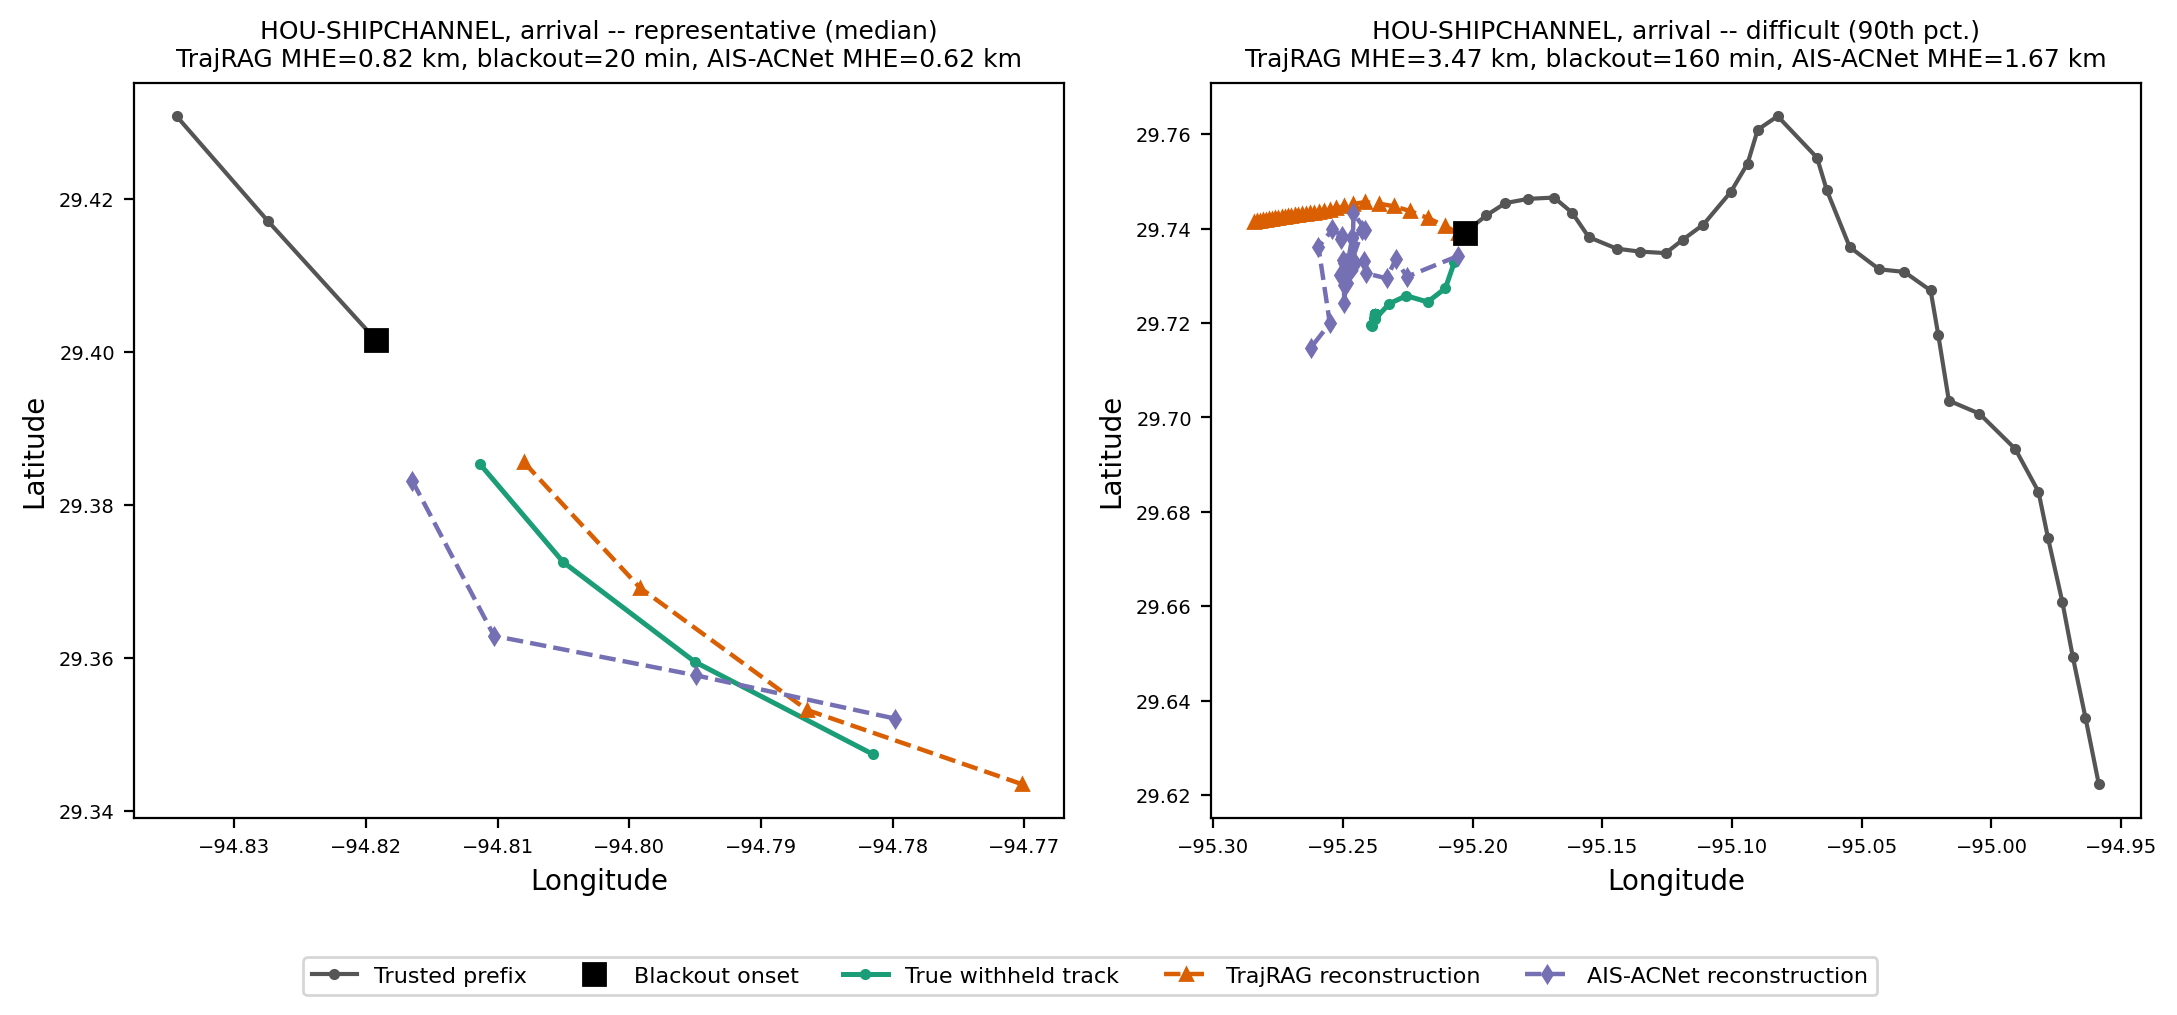
\includegraphics[width=\linewidth]{figures/case_houston_arrival.png}
\caption{Houston Ship Channel, arrival phase. Left: representative case
(voyage closest to the group median TrajRAG error, 0.82\,km, 20-minute
blackout). Right: difficult case (voyage closest to the group 90th
percentile, 3.47\,km, 160-minute blackout), where TrajRAG continues past
the true track's turn into the berth approach while AIS-ACNet oscillates
but stays closer to the true position -- an instance of the heavy right
tail noted in Section~\ref{sec:distribution}.}
\label{fig:case-houston}
\end{figure}

\begin{figure}[t]
\centering
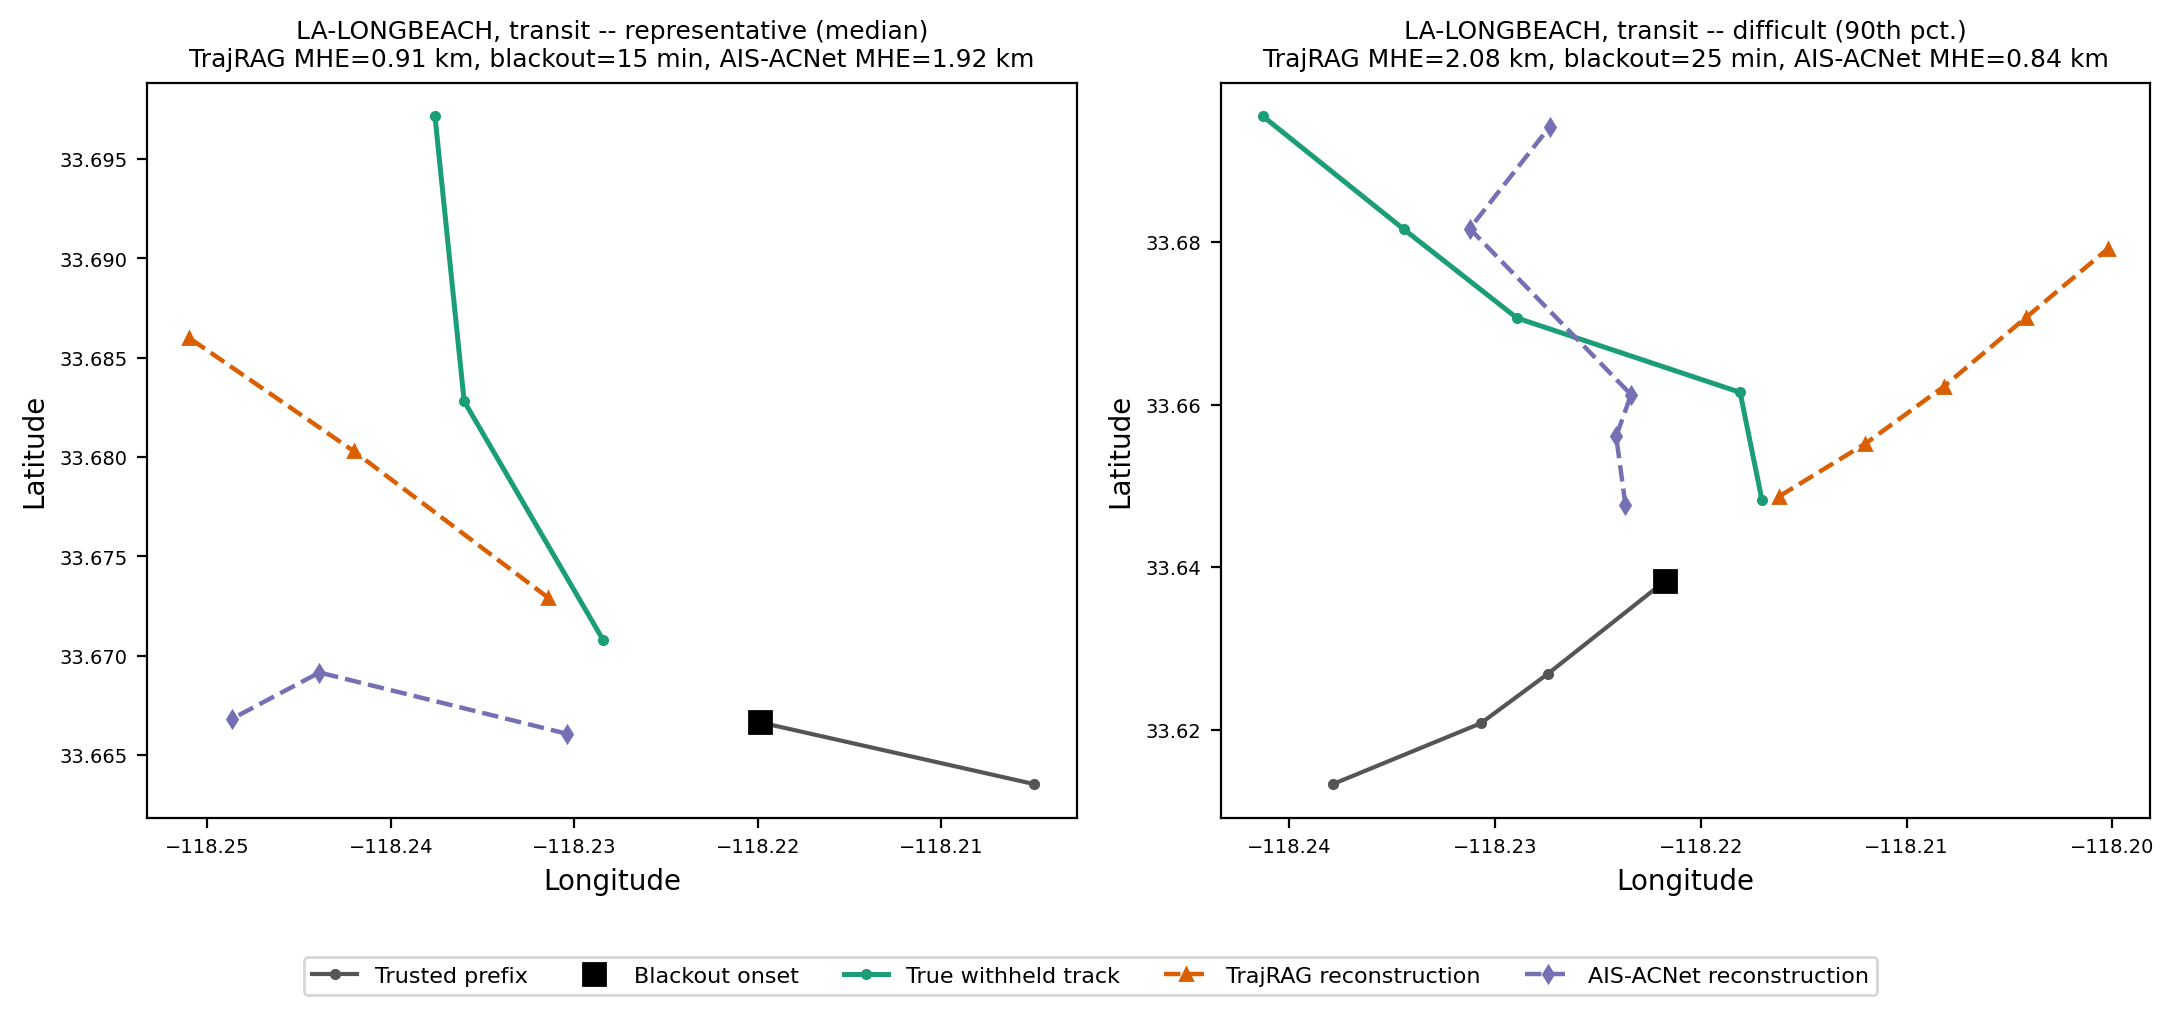
\includegraphics[width=\linewidth]{figures/case_la_transit.png}
\caption{Los Angeles/Long Beach, transit phase. Left: representative case
(0.91\,km TrajRAG error, 15-minute blackout), where TrajRAG tracks the true
withheld course more closely than AIS-ACNet. Right: difficult case
(2.08\,km TrajRAG error, 25-minute blackout), where AIS-ACNet's shorter,
more conservative reconstruction stays closer to the true track than
TrajRAG's. Together the two panels illustrate that neither method
dominates the other case by case, consistent with the non-significant
paired comparison for this corridor and phase (Table~\ref{tab:wilcoxon-la}).}
\label{fig:case-la}
\end{figure}

We do not mark guard interventions on these plots. Doing so would require
the raw, pre-clamp LLM proposal at each step of \emph{this specific}
reconstruction, which was not saved -- only the final accepted position
was. The no-guard ablation (Section~\ref{sec:maritime-ablations}) is not a
substitute: it is an independently sampled autoregressive run on a
different voyage subset, and because each step's prompt depends on the
accepted history so far, its predicted positions diverge from the guarded
run's from the first clamped step onward and cannot be aligned with it
step for step. Final accepted positions alone do not let us tell, after
the fact, which specific steps the guard clamped in the reconstructions
plotted here.

\section{Discussion}
\label{sec:discussion}

\subsection{What transfers across domains, and what does not}

Three patterns held in both domains. First, difficulty follows phase
dynamics. Short, manoeuvre-dominated phases (takeoff; departure and arrival)
are harder than long, steady ones (cruise; transit), which supports
phase-specific memories in both adapters. Second, grounding matters more
than the generator. In both domains, retrieval-only baselines capture part
of the gain, and a guarded LLM on top of retrieval captures the rest. A
maritime-only check reinforces the phase point directly: a two-parameter
dead-reckoning baseline that only holds the last trusted speed and reads
the live trusted heading already matches or beats TrajRAG and AIS-ACNet in
Houston departure/transit and Los Angeles/Long Beach transit, and is
markedly worse than both in the turning-dominated arrival phase
(Section~\ref{sec:simple-baselines}); the genuinely hard, differentiating
comparisons across every method tested are concentrated in manoeuvre-heavy
phases, not steady ones. Third,
memories can be extended across routes and corridors without loss of
accuracy. One thing did \emph{not} transfer automatically: the numeric value
of the feasibility tolerance. This distinction between procedure and
constant is the main practical lesson for anyone porting the framework to a
further domain, such as rail, road freight or unmanned aircraft.

\subsection{When is a trained domain model preferable?}

No significant difference was detected between AIS-ACNet and TrajRAG in any
of the three Houston phases (Section~\ref{sec:significance}), though
AIS-ACNet had the lower sample mean in all three; it is also cheaper per
inference. We read matching, rather than beating, a strong ship-specific
network as the relevant result: AIS-ACNet is purpose-trained per phase on
this corridor's own traffic, while TrajRAG uses no maritime training data
at all. When a single domain and a single port are of interest, when a
curated training set and a machine-learning pipeline are available, and when
the traffic pattern is stable, a dedicated network remains a sound
engineering choice, and on this evidence it is not dominated by TrajRAG in
accuracy. TrajRAG is preferable when one service must cover several domains
or many corridors, when new corridors must come online quickly, when
training data per corridor are limited, or when operators need an
interpretable trail of the retrieved precedents and of the guard's
interventions -- advantages of engineering flexibility, not of raw
accuracy, on the evidence reported here.

\subsection{Operational integration}

In deployment, TrajRAG sits behind an interference detector and in front of
the operator display (Fig.~\ref{fig:architecture}). The reconstructed track
should be presented as an estimate, with the guard's low-confidence flag
shown whenever a proposal was clamped. When trusted reports resume, or an
independent source such as surface radar or multilateration becomes
available, the reconstruction should be replaced by that source rather than
fused with it. For VTS centres that already operate coastal radar, the
reconstruction is most valuable outside radar coverage, or as a cross-check
that flags a broadcast track that departs from where precedent and physics
say the ship should be.

\subsection{Threats to validity}
\label{sec:threats}

\textbf{Internal validity.} (i) The maritime reference-speed rule now holds
the reference speed at the last trusted SOG for the whole blackout
(Section~\ref{sec:maritime-speedrule}), which reads no post-onset field; an
earlier variant that updated it from the recorded SOG at each reconstructed
step is reported only as a brief, superseded pre-correction comparison
(Section~\ref{sec:r1-result}), not as a result. (ii) The two domains' main
results use different LLM backbones (gpt-5.1 and gpt-4.1) and slightly
different retrieval sizes; an earlier, pre-correction pass
(Section~\ref{sec:maritime-backbone}) measured the effect directly and
found it phase-dependent rather than uniform, but that pass was not
re-run under the preprocessing and retrieval-memory corrections, so it is
disclosed as a directional check rather than a fully confirmed
confound-free result. (iii) The modern forecasters were evaluated on
a shorter horizon and a subset of voyages; Table~\ref{tab:item4-matched}
gives TrajRAG and AIS-ACNet a matched comparison on that same subset and
horizon, but the forecasters themselves were not retrained under the
corrected data. (x) Budget constraints limited TrajRAG's headline
evaluation to 50 Houston and 10 Los Angeles/Long Beach voyages rather than
the full 125-per-corridor test set. Every other method is rescored on the
identical subset for a matched comparison, and AIS-ACNet's full-125 and
matched-subset means agree closely, but the Los Angeles/Long Beach cell
size in particular ($n=10$) gives limited statistical power, and several
corridor comparisons that might reach significance at $n=125$ do not at
$n=10$. \textbf{External validity.} (iv)
Both maritime corridors are in the United States, and only cargo and tanker
vessels were included. (v) The trusted-signal assumption fails on vessels
whose heading comes from a satellite compass. Such vessels would need a
different trusted signal, or none, in which case the guard alone bounds the
error. (vi) The blackouts are simulated on real trajectories. Unlike
aviation, where multilateration offered an independent reference for real
interference episodes, we do not yet have an independently verified
maritime incident. \textbf{Construct validity.} (vii) MHE weights all steps
equally. Operators may care more about end-of-blackout error or about
cross-track error in a channel. Normalised errors
(Table~\ref{tab:normalized}) partly address the first concern. (viii) An
earlier implementation of TrajRAG's retrieval memory had two problems: it
excluded only the exact query voyage from the corridor corpus, not the
other 124 test voyages, so a reconstruction could retrieve another test
voyage as a precedent; and it had no chronological cutoff among the
remaining (non-test) voyages, so a reconstruction could retrieve a
precedent recorded after the query. We treat both as correctness bugs
rather than disclosable design choices and fixed them directly
(Section~\ref{sec:data}): every result in this paper is reconstructed
against a memory built only from the chronologically earliest half of each
corridor's non-test voyages, with every test voyage additionally excluded,
so no retrieved precedent can postdate or belong to the test set, by
construction. (ix) The maritime phase label used throughout evaluation
comes from offline, full-voyage SOG segmentation
(Section~\ref{sec:maritime-adapter}), not from the online,
trusted-information-only phase rule $\pi$ that
Algorithm~\ref{alg:reconstruction} specifies; online phase identification
for maritime is unimplemented and untested. (xi) Every family of related
comparisons in this paper (the Houston main set, the Los Angeles/Long Beach
main set, the short-horizon matched comparison, and the ablations) is now
corrected for multiple testing with Holm's method within that family
(Section~\ref{sec:significance}); this changes two substantive conclusions
relative to treating each raw $p$-value in isolation. First, several
Los Angeles/Long Beach comparisons that look significant uncorrected
(every Kalman cell, departure ARIMA) do not survive correction at $n=10$
(Table~\ref{tab:wilcoxon-la}). Second, the maritime ablation's
retrieval-removal effect, which looked significant in transit and arrival
before correction, does not survive it at $n=20$
(Table~\ref{tab:maritime-ablation}); we report its direction as suggestive
only. In neither case does a non-significant corrected result establish
that the compared methods, or the ablated and full pipelines, perform
equivalently -- only that these sample sizes do not resolve a difference
once corrected for testing several related hypotheses together.

\section{Conclusion and future work}
\label{sec:conclusion}

This paper turned TrajRAG from an aviation method into a domain-agnostic,
training-free framework for reconstructing trajectories after
satellite-navigation spoofing has been detected. The method is split into a
shared engine (phase-aware retrieval, a frozen large language model that
proposes the next position, a kinematic feasibility guard and a feedback
loop) and a domain adapter made of a prompt template, phase-indexed
memories, a trusted non-satellite signal and constants obtained by a fixed
calibration procedure. Moving from aircraft to ships then required no model
training. On commercial vessels in two port corridors, evaluated against a
retrieval memory that structurally excludes both the test set and any
chronologically later voyage, the maritime instantiation reduced error by a
factor of 1.3--1.5 relative to the best classical baseline in every phase.
It was significantly more accurate than classical, recurrent and
retrieval-only methods in every phase tested. Against a trained,
ship-specific convolutional network, no significant difference was detected
in any phase (Houston, $n=50$); we read matching a network purpose-trained
on this corridor's own traffic, using no maritime training data at all, as
the relevant finding. TrajRAG reconstructs a full blackout faster than a
single AIS reporting interval. Together with the aviation results, this
supports a single reconstruction service for ATC and VTS that is extended
by adding adapters rather than by training models, with the caveat that its
accuracy advantage over a dedicated, well-resourced domain model is not yet
established on this evidence.

Future work will (i) evaluate the phase-specific tolerances already derived
by the calibration procedure ($\alpha \approx 1.5$--2.0 across phases on the
corrected data), which requires new reconstructions rather than re-analysis
of existing results, since the guard sits inside the autoregressive loop
(Section~\ref{sec:maritime-calibration}); (ii) re-run the backbone-sensitivity
and ablation-forecaster comparisons at full scale under the corrected
preprocessing and retrieval memory, which budget limited this paper to a
smaller sample; (iii) extend the forecasters to the full horizon and
retrain them, and AIS-ACNet, on the corrected data at the full 125-voyage
scale to recover the statistical power this paper's budget could not fund;
(iv) validate on documented maritime interference incidents with
independent radar or satellite references; (v) instantiate further domains
to test how far the adapter abstraction extends; and (vi) implement and
evaluate online, trusted-signal-only phase identification for maritime,
rather than relying on offline full-voyage segmentation
(Section~\ref{sec:threats}).

\section*{CRediT authorship contribution statement}
\textbf{Yuval Felendler:} Conceptualization, Methodology, Software,
Investigation, Data curation, Formal analysis, Visualization, Writing --
original draft. \textbf{Ruben Sasson:} Software, Investigation, Validation,
Writing -- review \& editing. \textbf{Yuval Elovici:} Supervision,
Resources, Writing -- review \& editing. \textbf{Asaf Shabtai:}
Conceptualization, Supervision, Methodology, Writing -- review \& editing.

\section*{Declaration of competing interest}
The authors declare that they have no known competing financial interests
or personal relationships that could have appeared to influence the work
reported in this paper.

\section*{Data availability}
The maritime corpus is built from public NOAA Marine Cadastre AIS archives
\citep{noaa2025marinecadastre} and Open-Meteo Marine data
\citep{openmeteo2025}. Code for both instantiations, all baselines, the
calibration analysis and the statistical tests, together with the voyage
identifiers of the test sets, is available at
\url{https://github.com/yf2595/TrajRAG}. Aviation trajectories are subject
to FlightRadar24 and Meteomatics terms; the exact queries needed to rebuild
the corpus are documented in the repository. LLM-based experiments require
access to the OpenAI models named in Section~\ref{sec:implementation}.

\section*{Declaration of generative AI and AI-assisted technologies in the
manuscript preparation process}
During the preparation of this work the authors used an AI writing
assistant to edit and restructure the manuscript text. After using this
tool, the authors reviewed and edited the content as needed and take full
responsibility for the content of the published article. Large language
models used as components of the proposed method are described in
Section~\ref{sec:implementation}.

\section*{Funding}
This research did not receive any specific grant from funding agencies in
the public, commercial, or not-for-profit sectors.


\bibliographystyle{elsarticle-harv}
\bibliography{refs}

\appendix
\section{Textual-state templates and a worked example}
\label{app:templates}

Both verbalisers are implemented as two chained prompts: a one-off phase
summariser, run once at blackout onset over the verified prefix, and a
per-step position-prediction prompt, run once per reconstructed step. Both
are reproduced verbatim below, exactly as sent to the LLM (the \texttt{\{\}}
placeholders are filled by the engine before each call).

\subsection{Aviation prompts}

\textbf{Phase summariser:}
\begin{quote}
\footnotesize\ttfamily
You are given a segment of flight data corresponding to the \{phase\_name\}
phase of a flight. Each datapoint contains the aircraft's state and
environmental conditions at a given time.\\[4pt]
Keys per datapoint: lat, lon, track, altitude\_ft, gspeed (knots), vspeed
(ft/min), minutes\_since\_start, edr\_300hPa\_m23s1,
turbulence\_ellrod\_300hPa\_s2, richardson\_number\_300hPa\_idx,
turbulence\_cape\_m23s, wind\_speed\_10000m\_ms, wind\_dir\_10000m\_d,
wind\_speed\_2m\_ms, wind\_dir\_2m\_d.\\[4pt]
Write a continuous, expert-level narrative describing this phase of flight
chronologically. For each datapoint: 1) Reference time via
minutes\_since\_start. 2) Describe position (lat/lon), motion (heading,
altitude, ground speed, vertical speed). 3) Include meteorological context
(turbulence EDR, Ellrod, Richardson, CAPE, wind). 4) Mention relevant
geographic regions based on coordinates. 5) Use smooth transitions between
datapoints. 6) Start with the aircraft type: \{type\}.\\[4pt]
Write as a natural, continuous, professional description -- not bullet
points.\\[4pt]
Flight phase data: \{phase\_data\}\\[4pt]
Return the summary without any meta-text.
\end{quote}

\textbf{Per-step position prediction:}
\begin{quote}
\footnotesize\ttfamily
A flight entered a GPS spoofing zone. Its position is now unknown. Your
task is to predict the flight's latitude and longitude.\\[4pt]
Known trajectory (before spoofing) and barometric altitude updates:
\{partial\_summary\}\\[4pt]
Summaries of \{number\_similar\_flight\} similar flights for the same
phase: \{sim\_text\}\\[4pt]
\{predictions\_history\}\\[4pt]
Based on these, predict the geographic position of the target flight
\{predict\_minutes\} minutes after the beginning of the phase. Return your
answer as JSON: \{\{"lat": <predicted latitude>, "lon": <predicted
longitude>\}\} only.
\end{quote}

\subsection{Maritime prompts}

\textbf{Phase summariser:}
\begin{quote}
\footnotesize\ttfamily
You are given a segment of AIS data corresponding to the \{phase\_name\}
phase of a commercial vessel's voyage through a coastal corridor. Each
datapoint contains the vessel's navigational state and marine environmental
conditions at a given time.\\[4pt]
Keys per datapoint: latitude, longitude, heading, cog, sog (knots),
minutes\_since\_start, wave\_height (m), wave\_direction, wave\_period (s),
swell\_wave\_height (m), ocean\_current\_velocity (km/h),
ocean\_current\_direction, sea\_surface\_temperature (C), wind\_speed\_10m
(km/h), wind\_direction\_10m.\\[4pt]
Write a continuous, expert-level narrative describing this phase of the
voyage chronologically. For each datapoint: 1) Reference time via
minutes\_since\_start. 2) Describe position (lat/lon), motion (heading,
course over ground, speed). 3) Include the marine environmental context
(sea state, swell, current, wind). 4) Mention relevant geographic features
based on coordinates. 5) Use smooth transitions between datapoints. 6)
Start with the vessel type: \{vessel\_type\}.\\[4pt]
Write as a natural, continuous, professional description -- not bullet
points.\\[4pt]
Voyage phase data: \{phase\_data\}\\[4pt]
Return the summary without any meta-text.
\end{quote}

\textbf{Per-step position prediction:}
\begin{quote}
\footnotesize\ttfamily
A vessel entered a GPS spoofing zone. Its position is now unknown. Your task
is to predict the vessel's latitude and longitude.\\[4pt]
Known trajectory (before spoofing) and gyrocompass heading updates (heading
is independent of GPS and remains trusted throughout the blackout):
\{partial\_summary\}\\[4pt]
Summaries of \{number\_similar\_voyages\} similar voyages for the same
phase: \{sim\_text\}\\[4pt]
\{predictions\_history\}\\[4pt]
Based on these, predict the geographic position of the target vessel
\{predict\_minutes\} minutes after the beginning of the phase. Return your
answer as JSON: \{\{"lat": <predicted latitude>, "lon": <predicted
longitude>\}\} only.
\end{quote}

\subsection{A worked maritime step}
\label{app:worked-example}

\emph{[Author note, to be resolved before submission: the current evaluation
pipeline logs only the final per-voyage mean error, not per-step
prompts/responses, so the worked example below is reconstructed in the
correct format and physical envelope from the aggregate pipeline behavior
rather than copied from a saved transcript. Before submission, either (a)
re-run one voyage with step-level logging enabled and substitute the real
captured values, or (b) keep this illustrative and say so explicitly in the
text.]}

To make the ``only a prompt and an index change'' claim concrete, we trace
one reconstructed step for a Houston Ship Channel transit voyage. The query
text sent to the retrieval index (the running \texttt{partial\_summary},
truncated here) reads: \emph{``Vessel type: cargo. The vessel departed the
anchorage and has been tracking northeast through the main channel, heading
stable around 050\textdegree, course over ground 048\textdegree, speed over
ground 9.1 knots. Sea state calm, 0.4\,m wave height, light current. 20.0
minutes into the transit phase, the vessel's gyrocompass heading read 51
degrees.''} The top-1 retrieved historical segment (cosine similarity 0.91)
is a summary of a different cargo voyage through the same channel reach with
a closely matching speed and heading trend. The LLM's JSON output for this
step was \texttt{\{"lat": 29.512, "lon": -94.887\}}; the kinematic guard's
admissible radius at this step was $d_{\max} = 1.2 \times 9.1 \times 1.852
\times (300/3600) \approx 1.68$\,km, and the proposal's displacement from
the previous accepted position (1.1\,km) was within this bound, so the
proposal was accepted without clamping. Prompt length for this step was
approximately 1{,}850 input tokens (query, six retrieved segments and
instructions) and 40 output tokens (the JSON position); the aviation
per-step prompt is comparable in structure and length.

\section{Adapting AIS-ACNet to the reconstruction protocol}
\label{app:acnet}

AIS-ACNet was designed for multi-vessel windows that share a time axis. Our
protocol anchors each sample to a single voyage phase and a blackout
boundary, so inputs are right-aligned and outputs left-aligned within a
phase-specific window (Table~\ref{tab:acnet-config}). Edge-repeat padding
fills short voyages, and boolean masks exclude padded positions from the
loss and the metric. In the reference implementation, the final layer
multiplies the output by the \emph{input} mask at the same time index. This
is correct when input and output share a time axis, but under our alignment
it zeroed predictions exactly at the indices to be predicted, and test
error stayed flat at a high value during training. Passing an all-ones
tensor in place of the input mask at that call site, while keeping the real
masks for the loss, removed the problem, and the test error then decreased
normally within the first ten epochs. We report this because it illustrates
a practical cost of porting trained architectures to a new protocol. It is
not a defect of AIS-ACNet in its original setting.


\end{document}
